\subsection{Irreducible backgrounds}

\textcolor{red}{We are completing the update of the impact of theoretical uncertainties on the irreducible background predictions, it will be included in the next update of the AN.}

%\subsection{\texorpdfstring{$\ttbar\gamma^*$ and $\ttbar\gamma$}{tt gamma* and tt gamma} backgrounds} %%% subsections have been merged
Irreducible backgrounds from $\ttbar\PW$, $\ttbar\Z$ and $\ttbar\PW\PW$, are estimated from
simulated events. The 2015 BDT outputs are used here as for the signal modelling,
and will be udpated in later versions of this note.
Just like for the signal, corrections are applied for the different performance
the individual physics objects between data and simulation measured in
control regions in data. The effect of the JEC uncertainties on the
final discriminator shapes is shown for $\ttbar\PW$, $\ttbar\Z$ in Fig.~\ref{fig:TTVJEConBDTshape2lss} and Fig.~\ref{fig:TTVJEConBDTshape3l}.

\begin{figure}[htb]
	\centering 
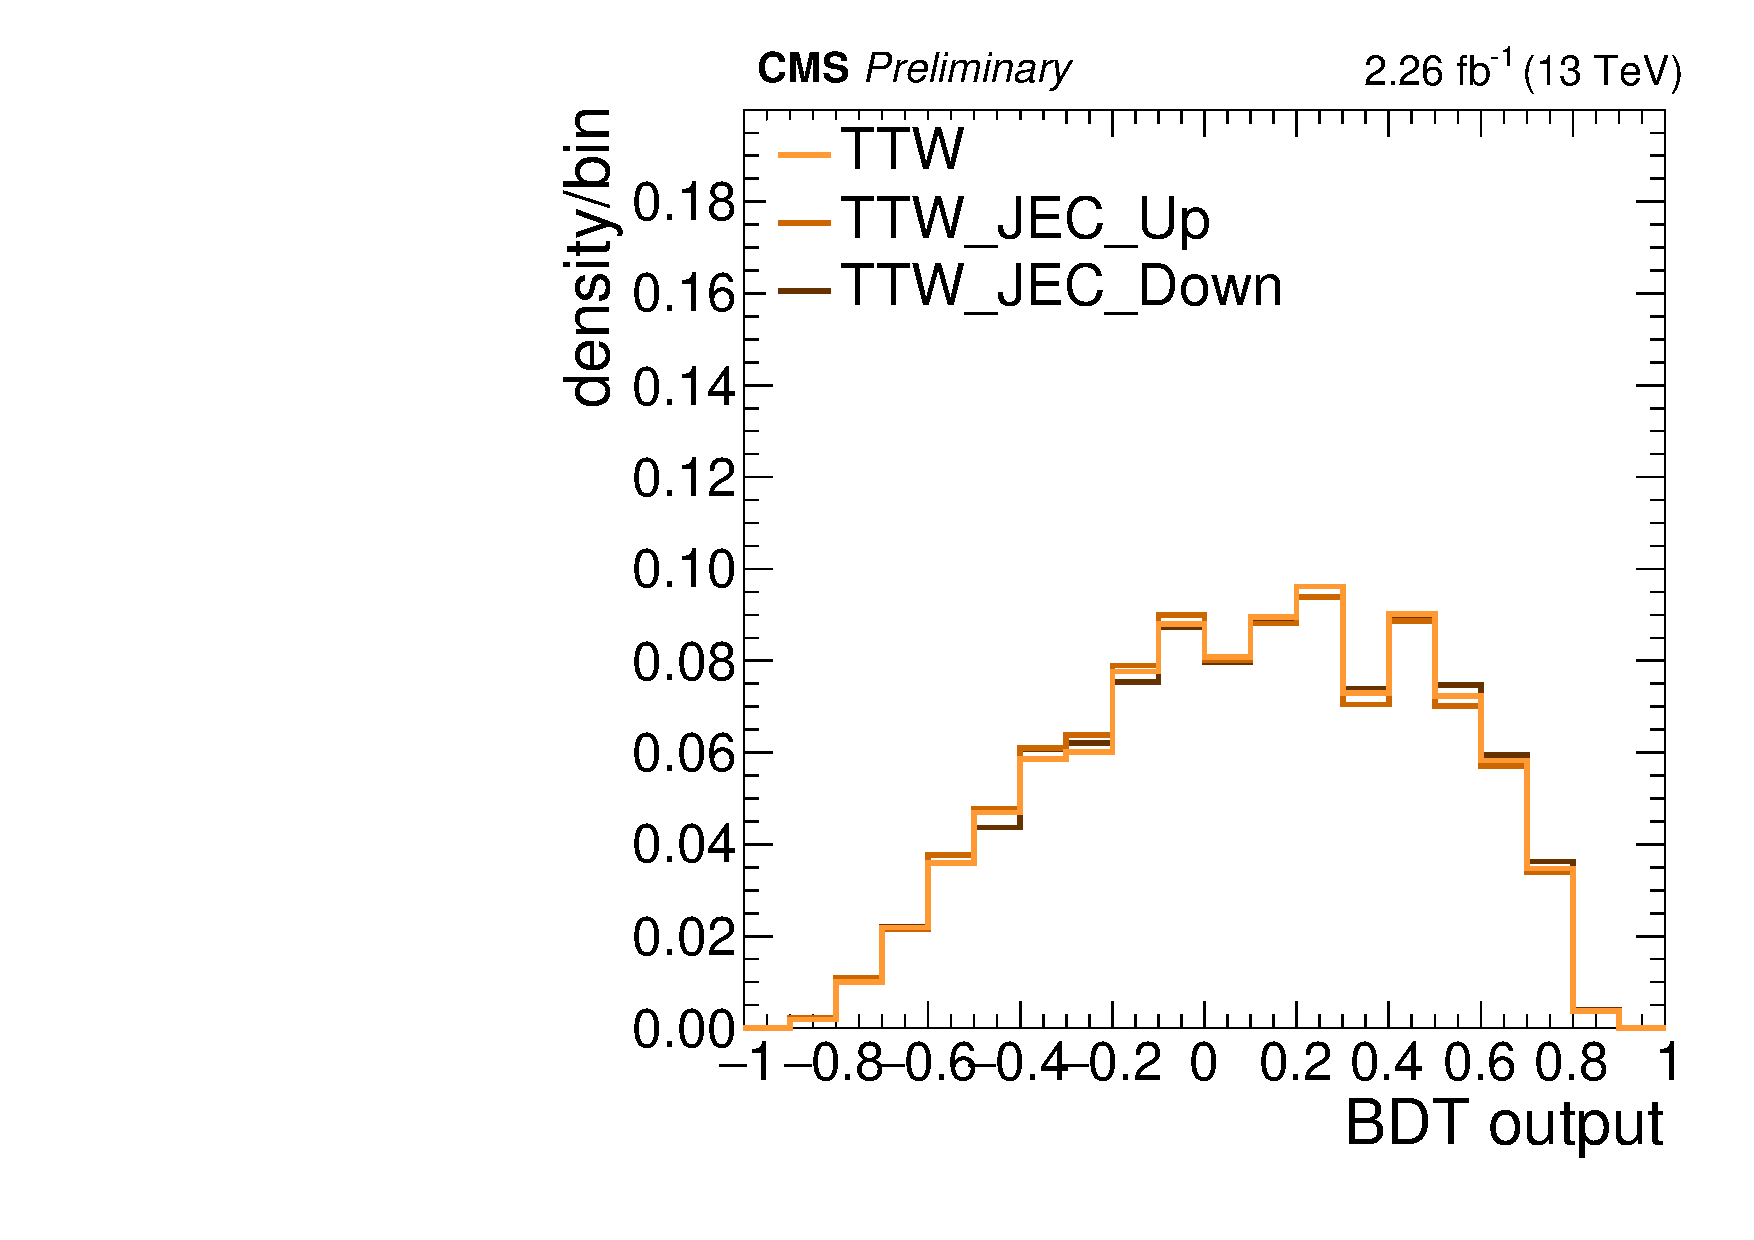
\includegraphics[width=0.35\textwidth]{plots_irreduciblebkg/2lss/JEC_ttW/kinMVA_2lss_ttbar}
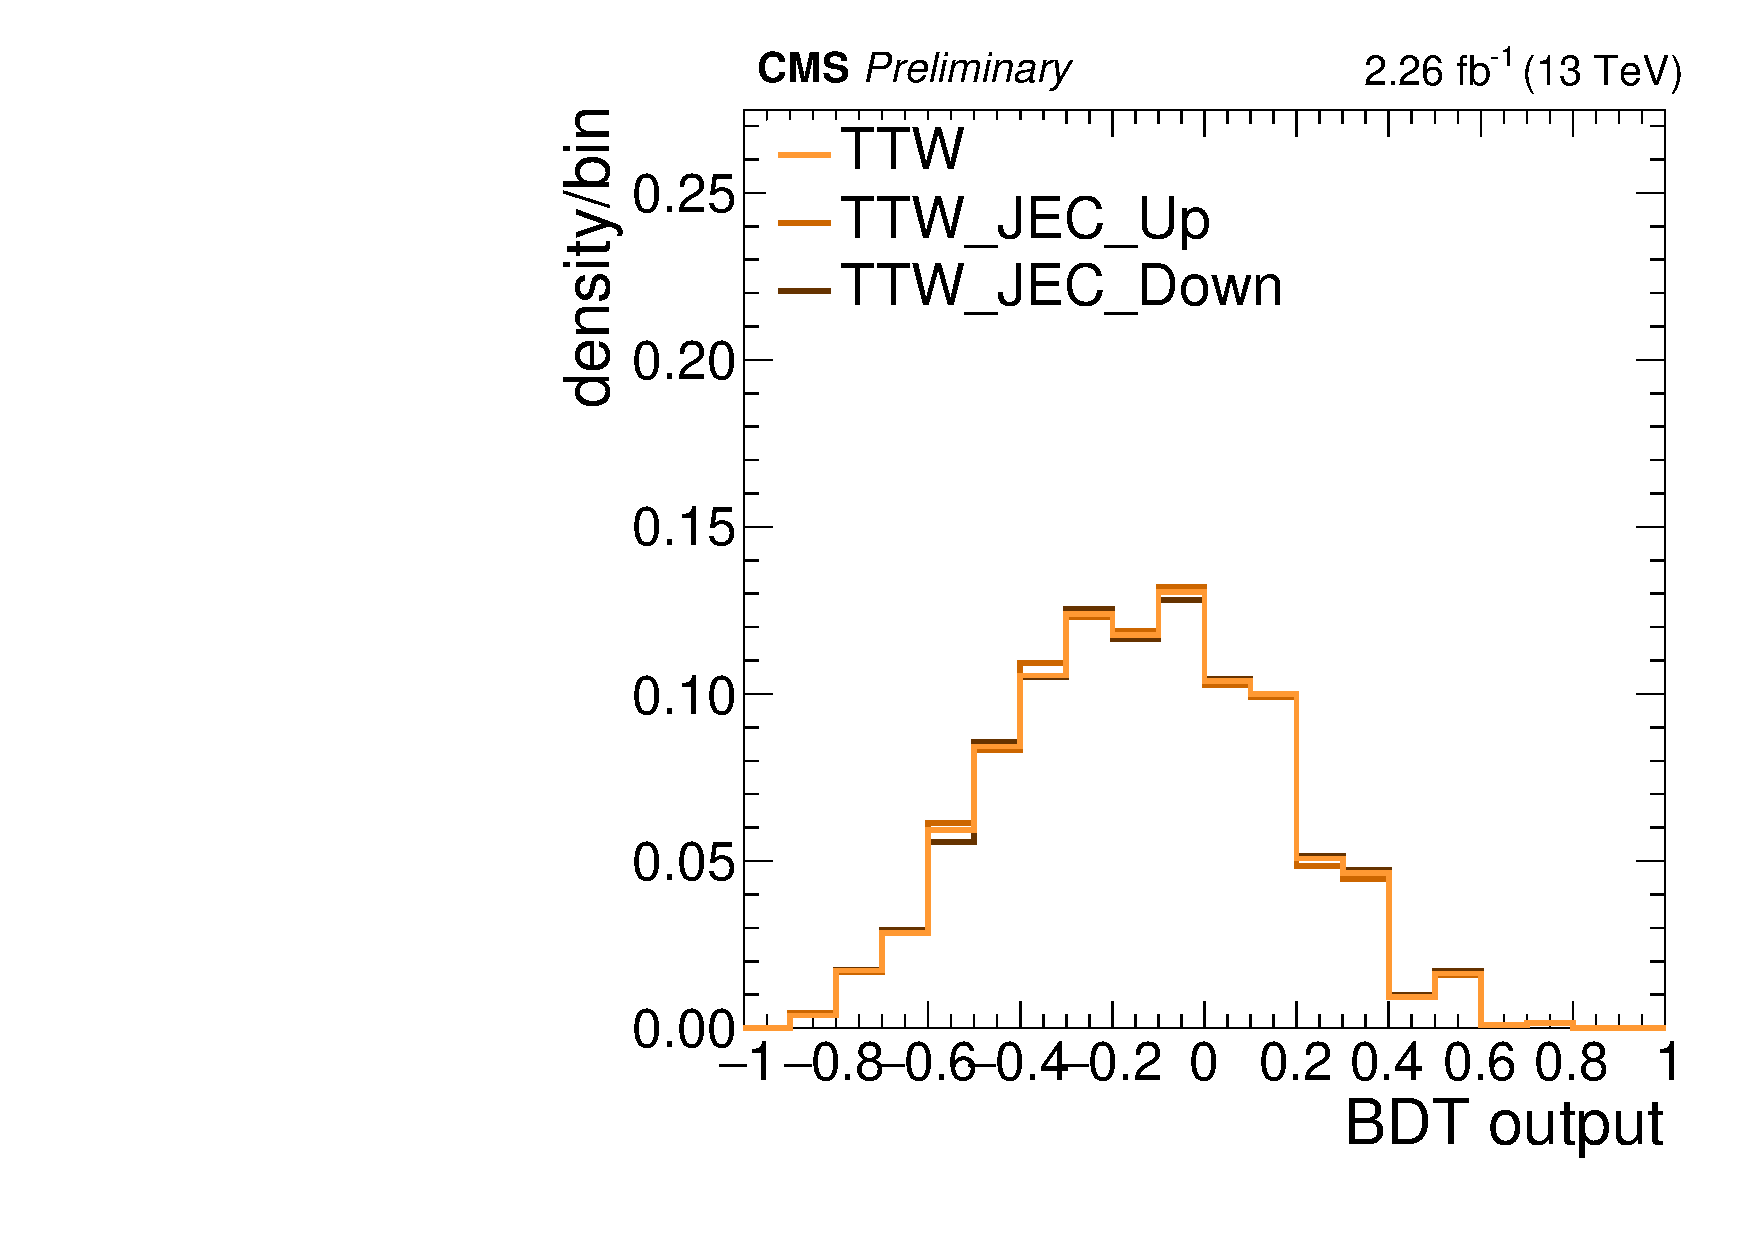
\includegraphics[width=0.35\textwidth]{plots_irreduciblebkg/2lss/JEC_ttW/kinMVA_2lss_ttV}
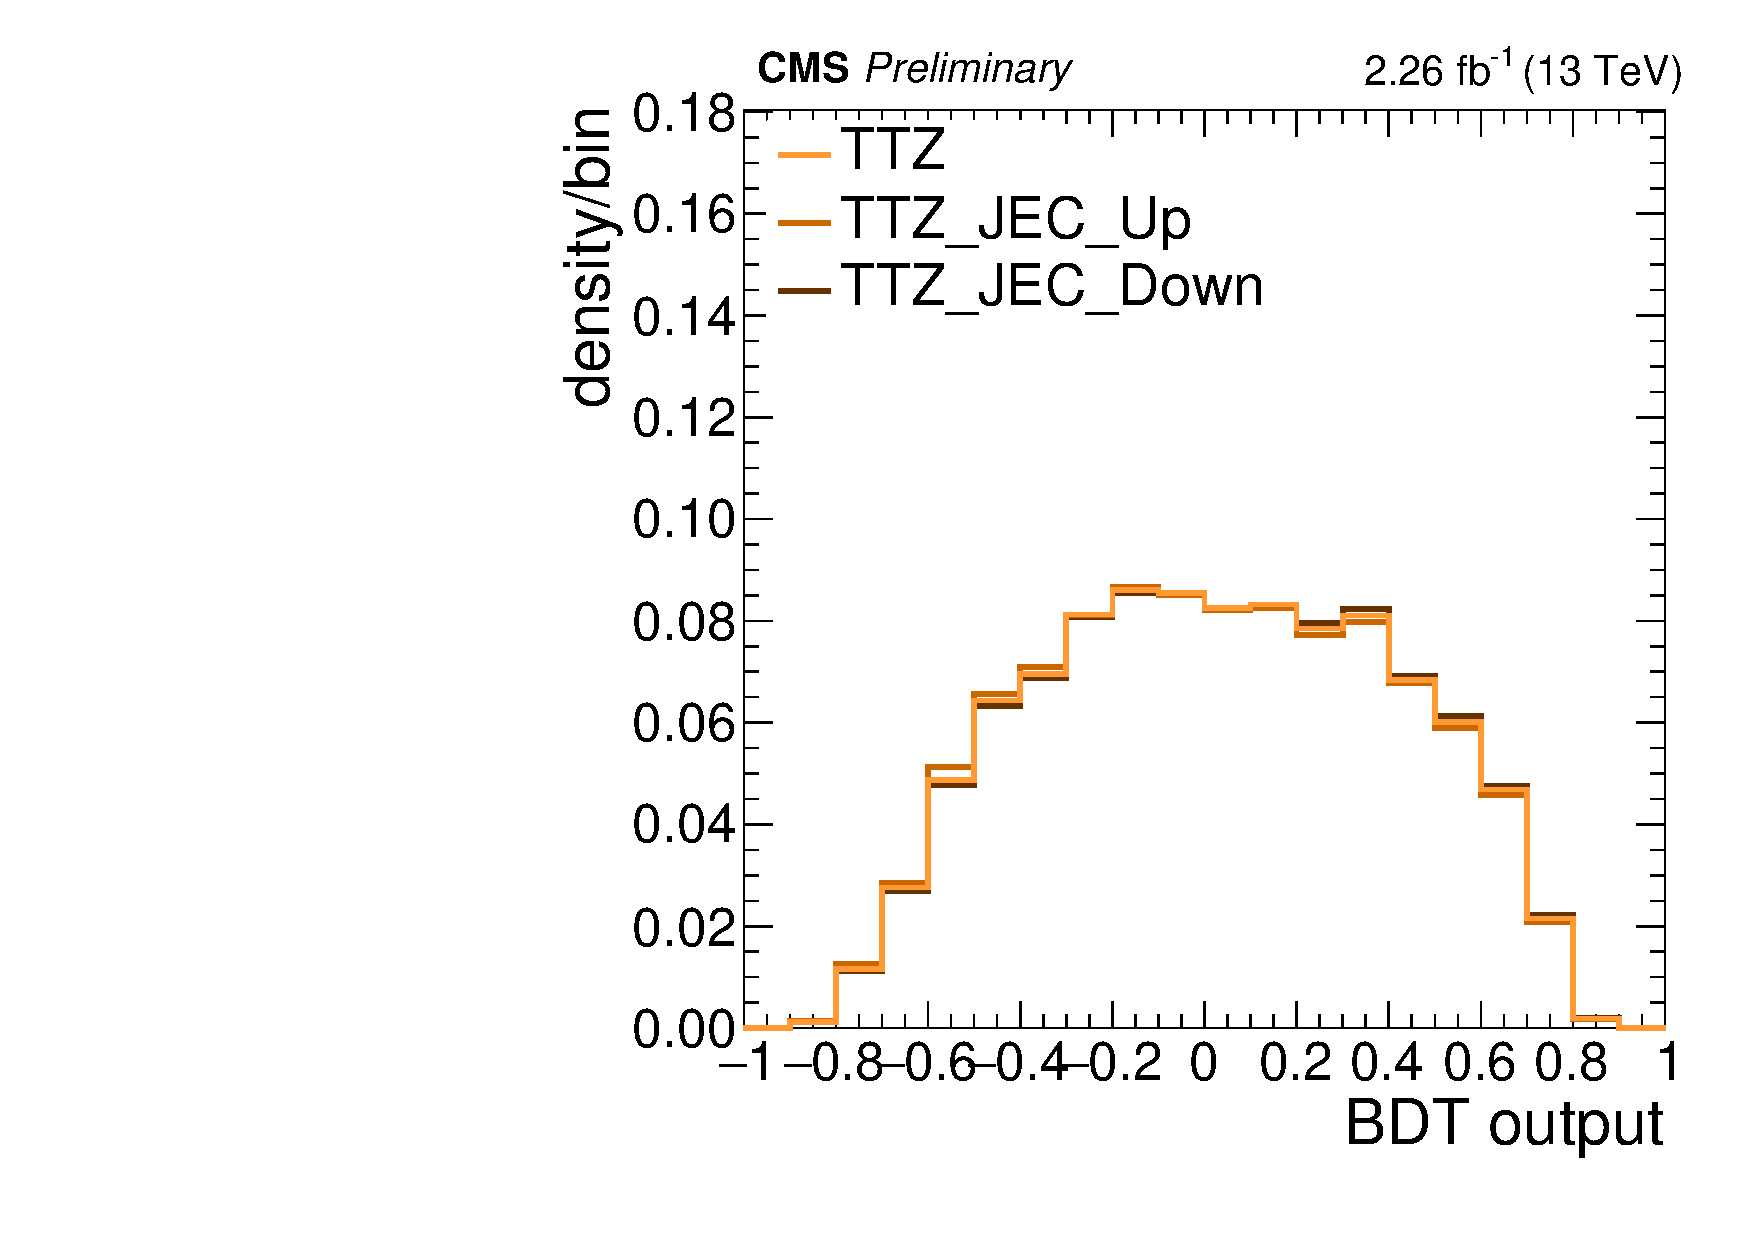
\includegraphics[width=0.35\textwidth]{plots_irreduciblebkg/2lss/JEC_ttZ/kinMVA_2lss_ttbar}
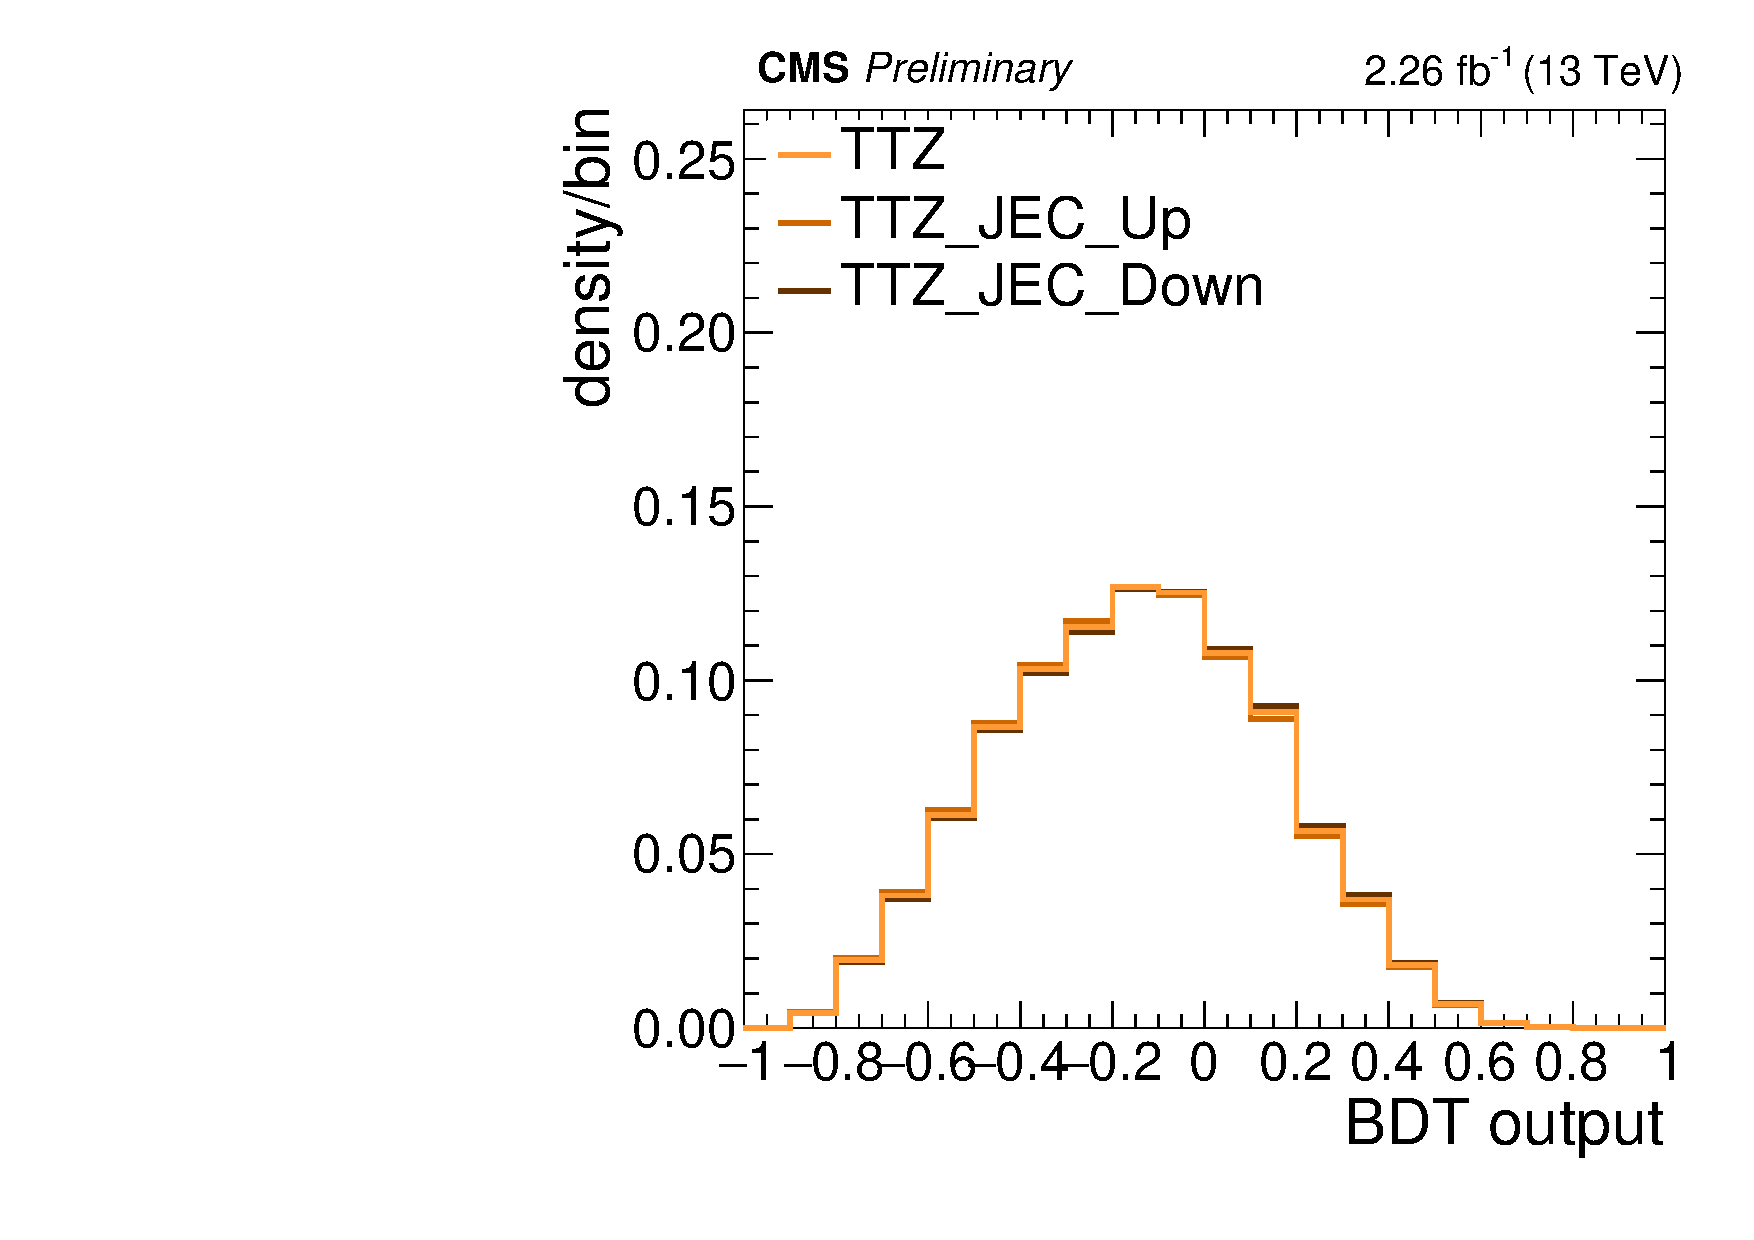
\includegraphics[width=0.35\textwidth]{plots_irreduciblebkg/2lss/JEC_ttZ/kinMVA_2lss_ttV}
	\caption{The BDT output distribution of the ttW and ttZ, shown for the training against ttbar 
	(left) and ttV (right) in the two same sign leptons final state, with the jet energy scale 
	variations of one standard deviation included in order to estimate the shape uncertainties.}
	\label{fig:TTVJEConBDTshape2lss}
\end{figure}

\begin{figure}[htb]
	\centering 
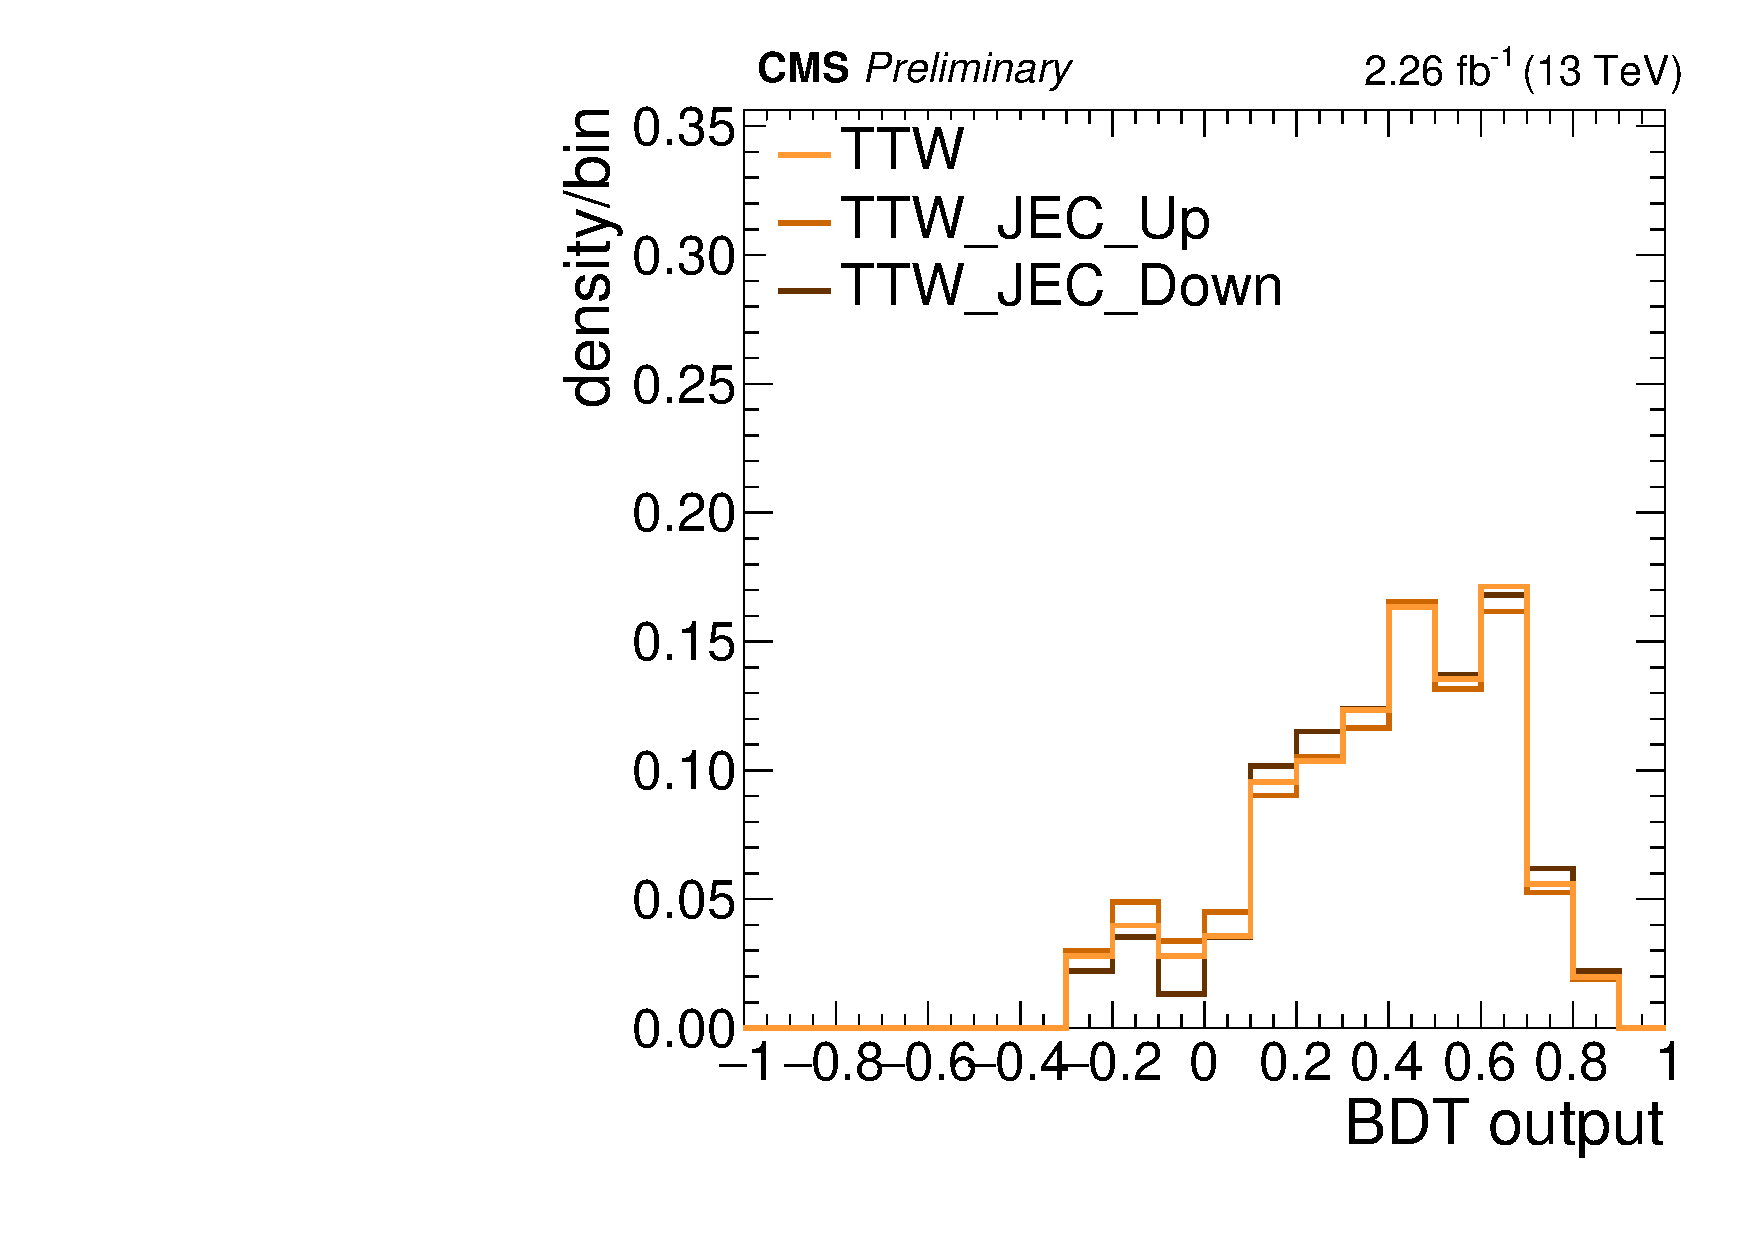
\includegraphics[width=0.35\textwidth]{plots_irreduciblebkg/3l/JEC_ttW/kinMVA_3l_ttbar}
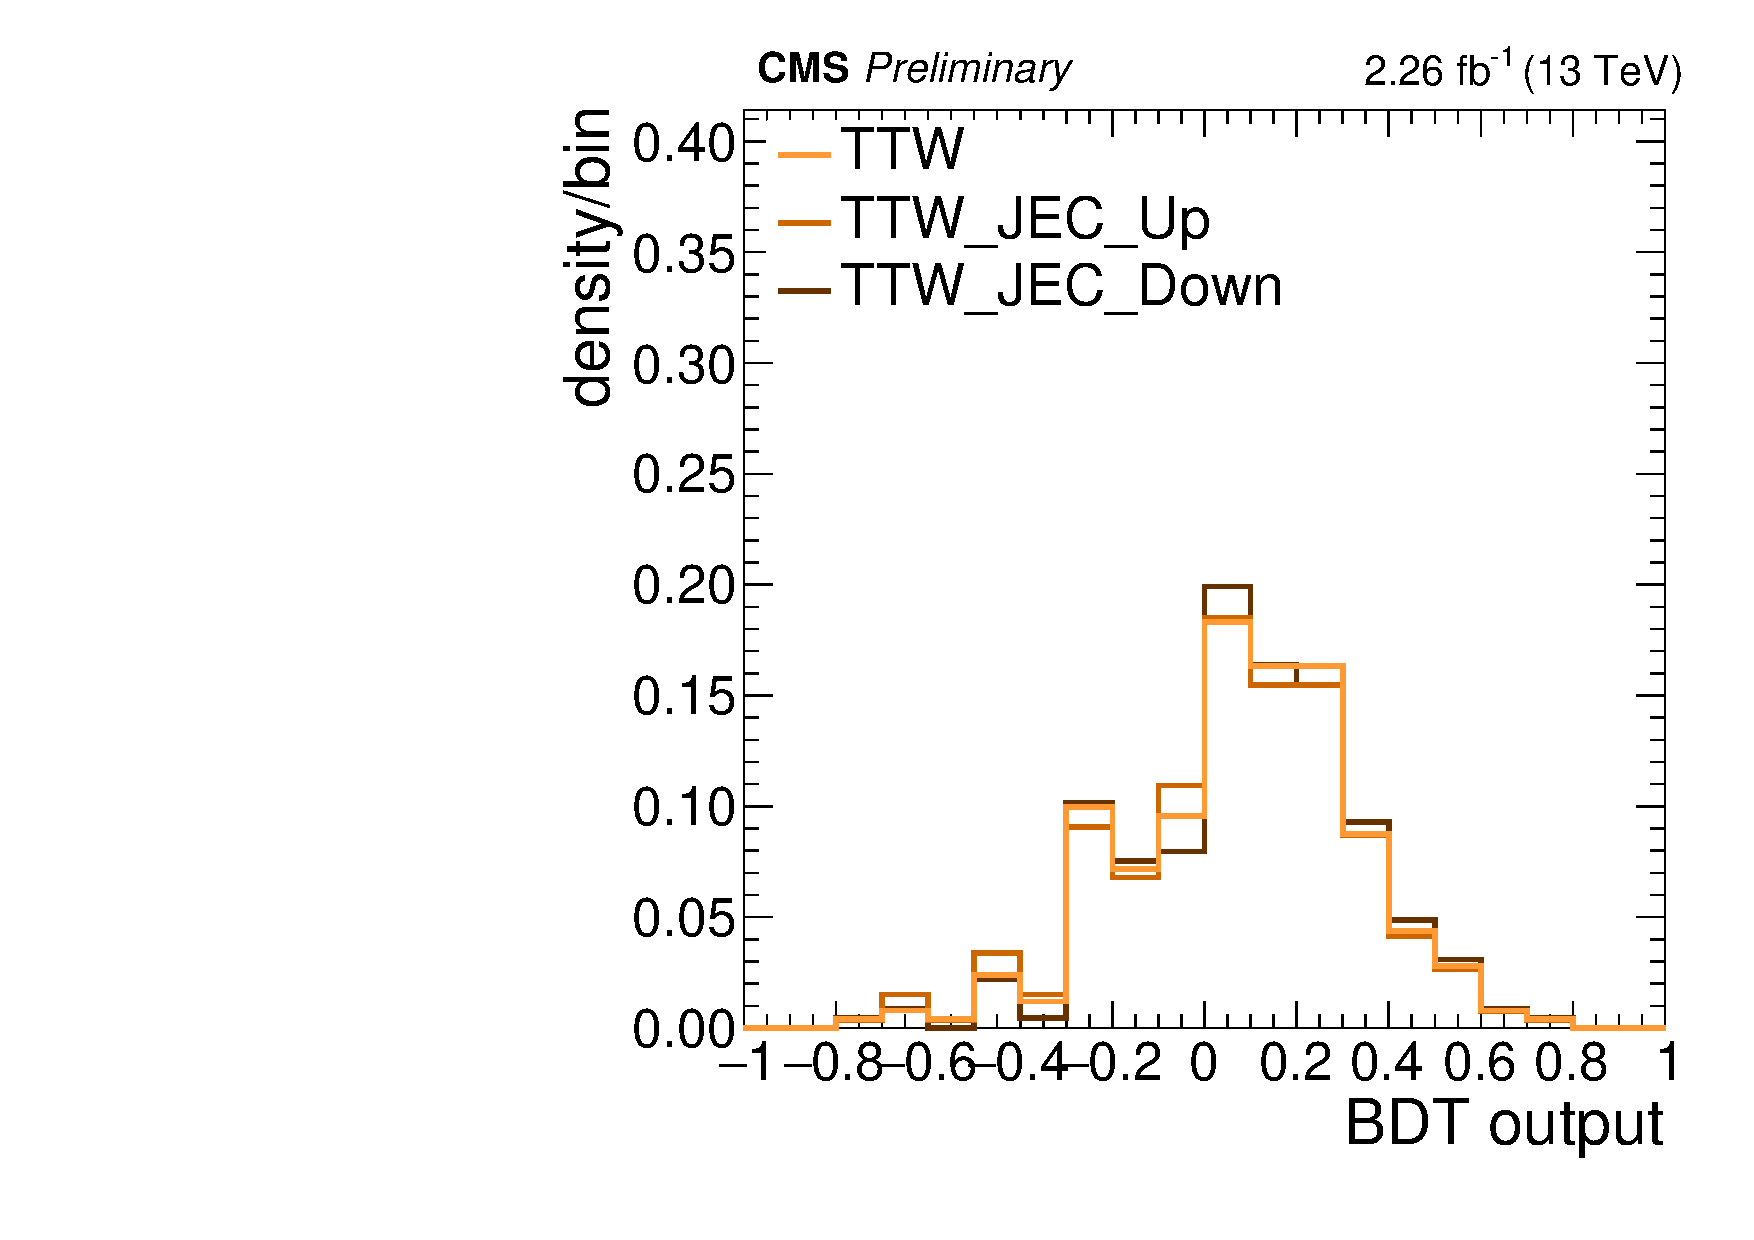
\includegraphics[width=0.35\textwidth]{plots_irreduciblebkg/3l/JEC_ttW/kinMVA_3l_ttV}
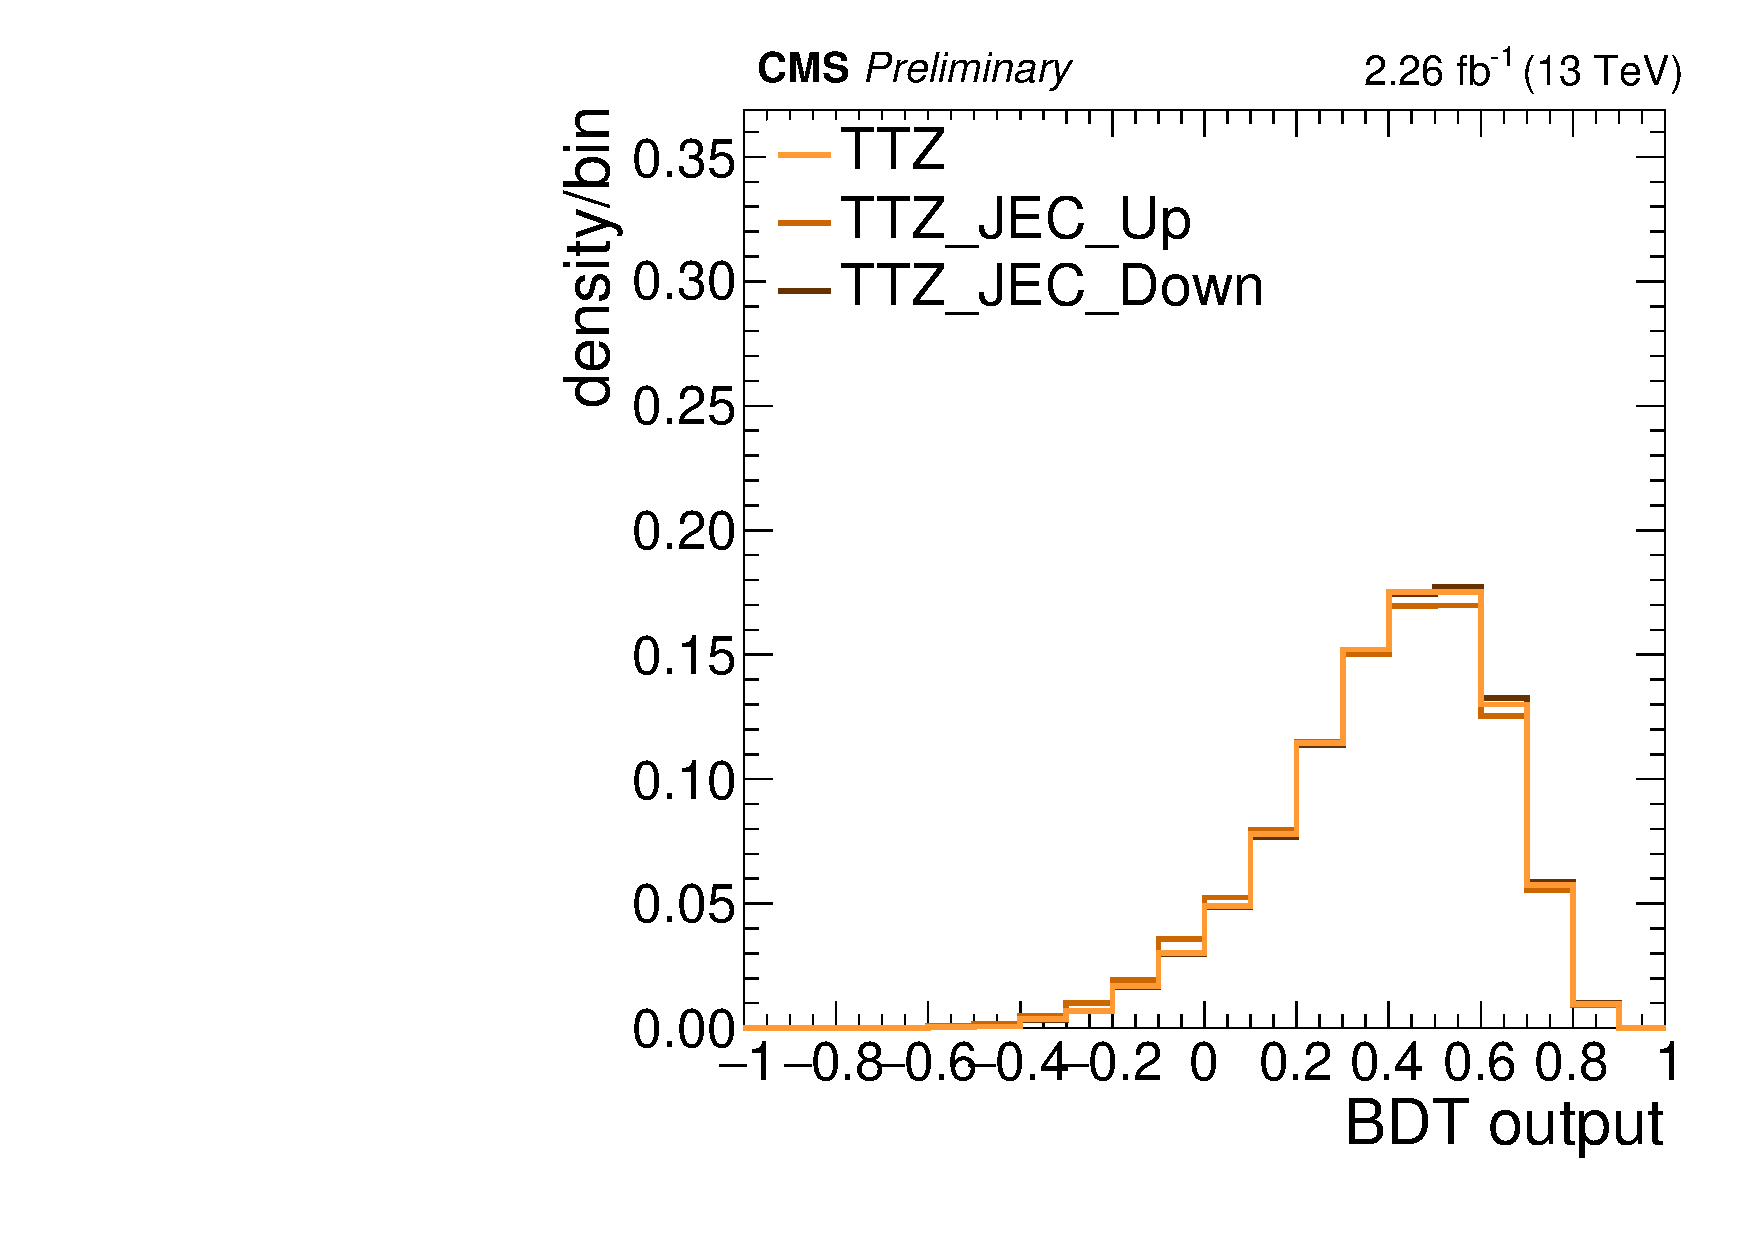
\includegraphics[width=0.35\textwidth]{plots_irreduciblebkg/3l/JEC_ttZ/kinMVA_3l_ttbar}
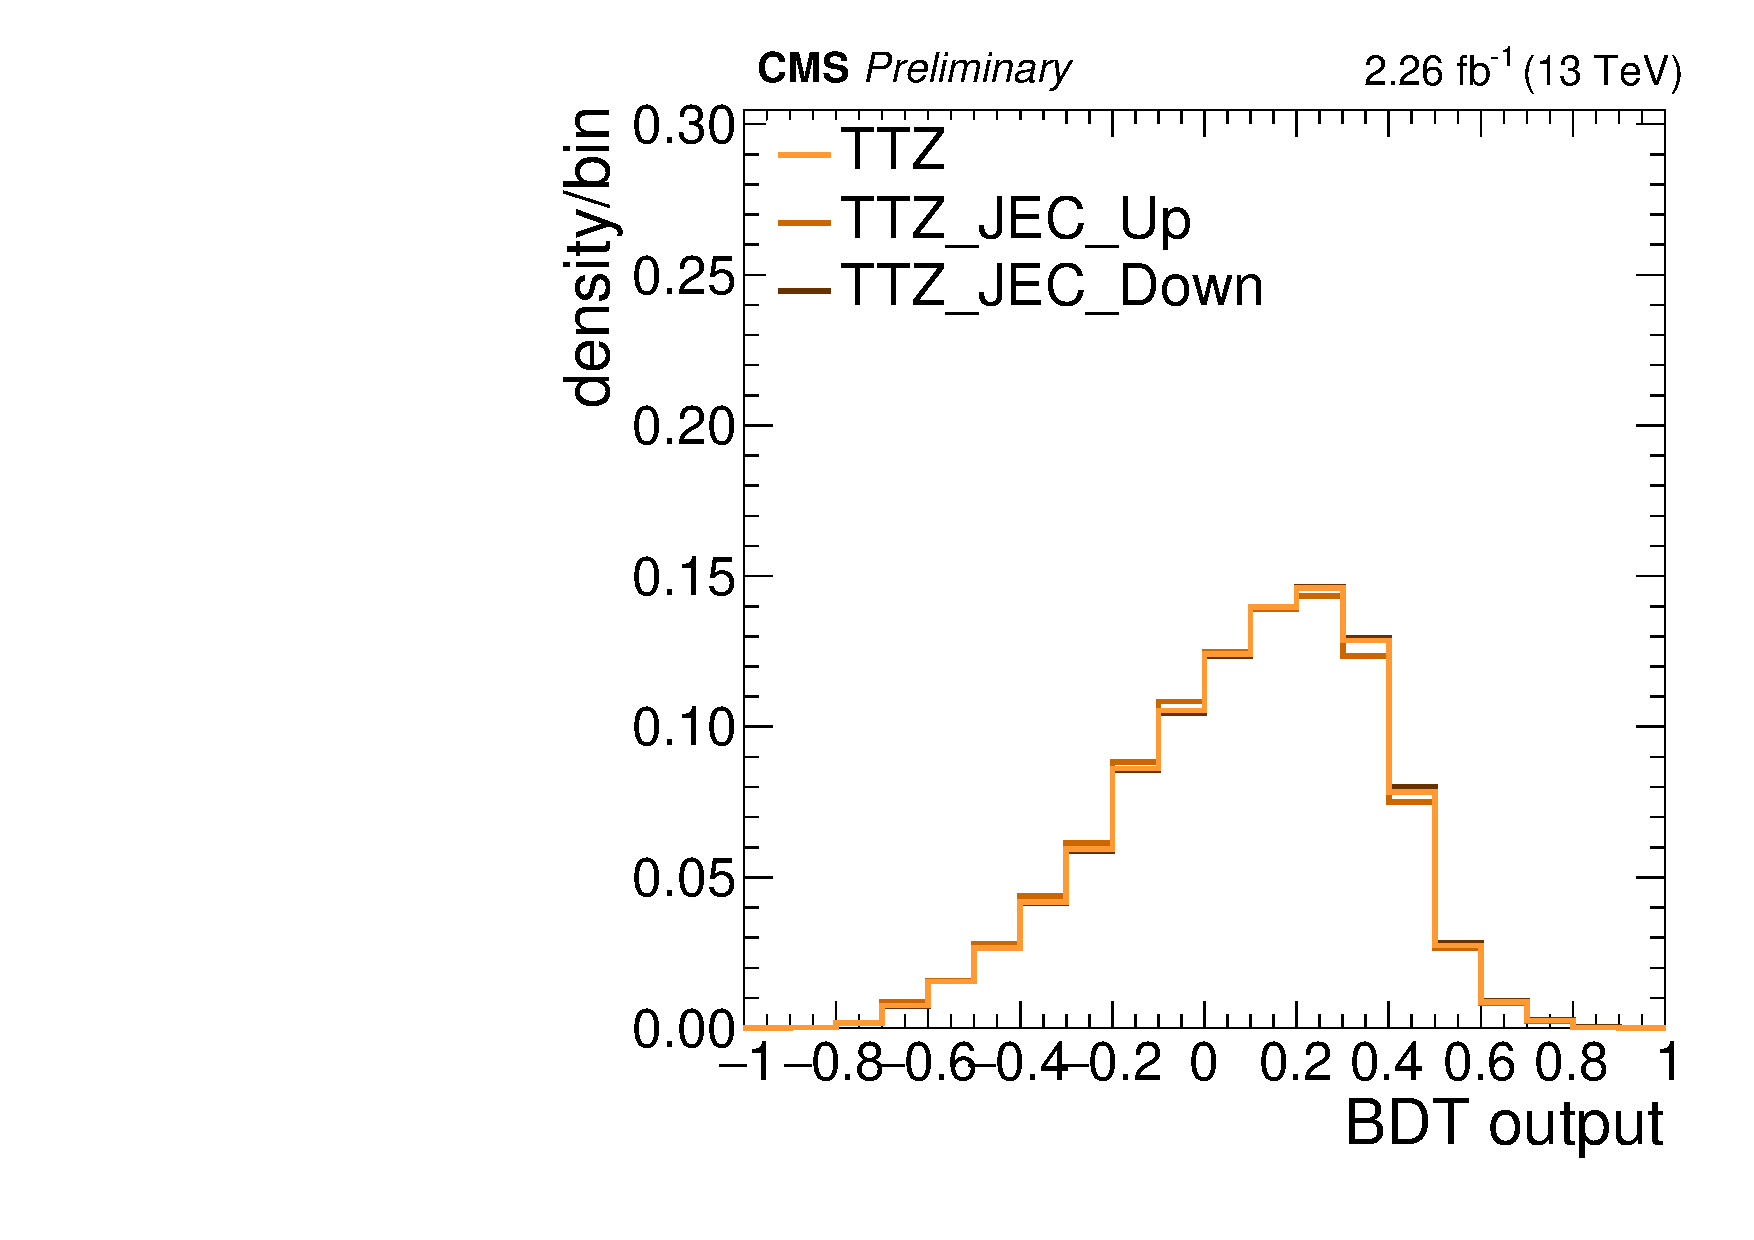
\includegraphics[width=0.35\textwidth]{plots_irreduciblebkg/3l/JEC_ttZ/kinMVA_3l_ttV}
	\caption{The BDT output distribution of the ttW and ttZ, shown for the training against ttbar 
	(left) and ttV (right) in the three lepton final state, with the jet energy scale 
	variations of one standard deviation included in order to estimate the shape uncertainties.}
	\label{fig:TTVJEConBDTshape3l}
\end{figure}



In the RunI analysis, the contribution of the $\ttbar\PW\PW$ process was found to be
at least an order of magnitude smaller than $\ttbar\PW$ and
$\ttbar\Z$. At 13 TeV, NLO (arXiv 1405.0301 table 6), the cross section is a factor of ~5 higher than at 8 TeV (partially because of the k factor as at 8 TeV we only had LO, and 13 TeV NLO/LO ~ 1.5). Therefore if it was negligible at 8 TeV it still is. 

The inclusive production cross sections for the $\ttbar\PW$ and $\ttbar\Z$ processes are taken
from the latest NLO computation, with theoretical uncertainties from unknown higher
orders of $12\%$ and $10\%$ respectively, and uncertainties from the knowledge of the parton
density functions and $\alpha_{s}$ of $2\%$ and $3\%$ respectively~\cite{YR4}.\\
In addition to the overall normalisation, systematic uncertainties of theoretical origin on the
distribution of the events in the final discriminating variables are considered, estimated
conventionally by varying the normalisation and factorisation scales up and down by a factor of two and
matching threshold between matrix element and parton shower. These
results are shown both for $\ttbar\PW$ and $\ttbar\Z$ in
Fig.~\ref{fig:TTVScaleonBDTshape2lss} and
~\ref{fig:TTVScaleonBDTshape3l}.
In the current version of the results the shape uncertainties on the BDTs output are of the order of $2\%$ to $4\%$.

\begin{figure}[htb]
	\centering 
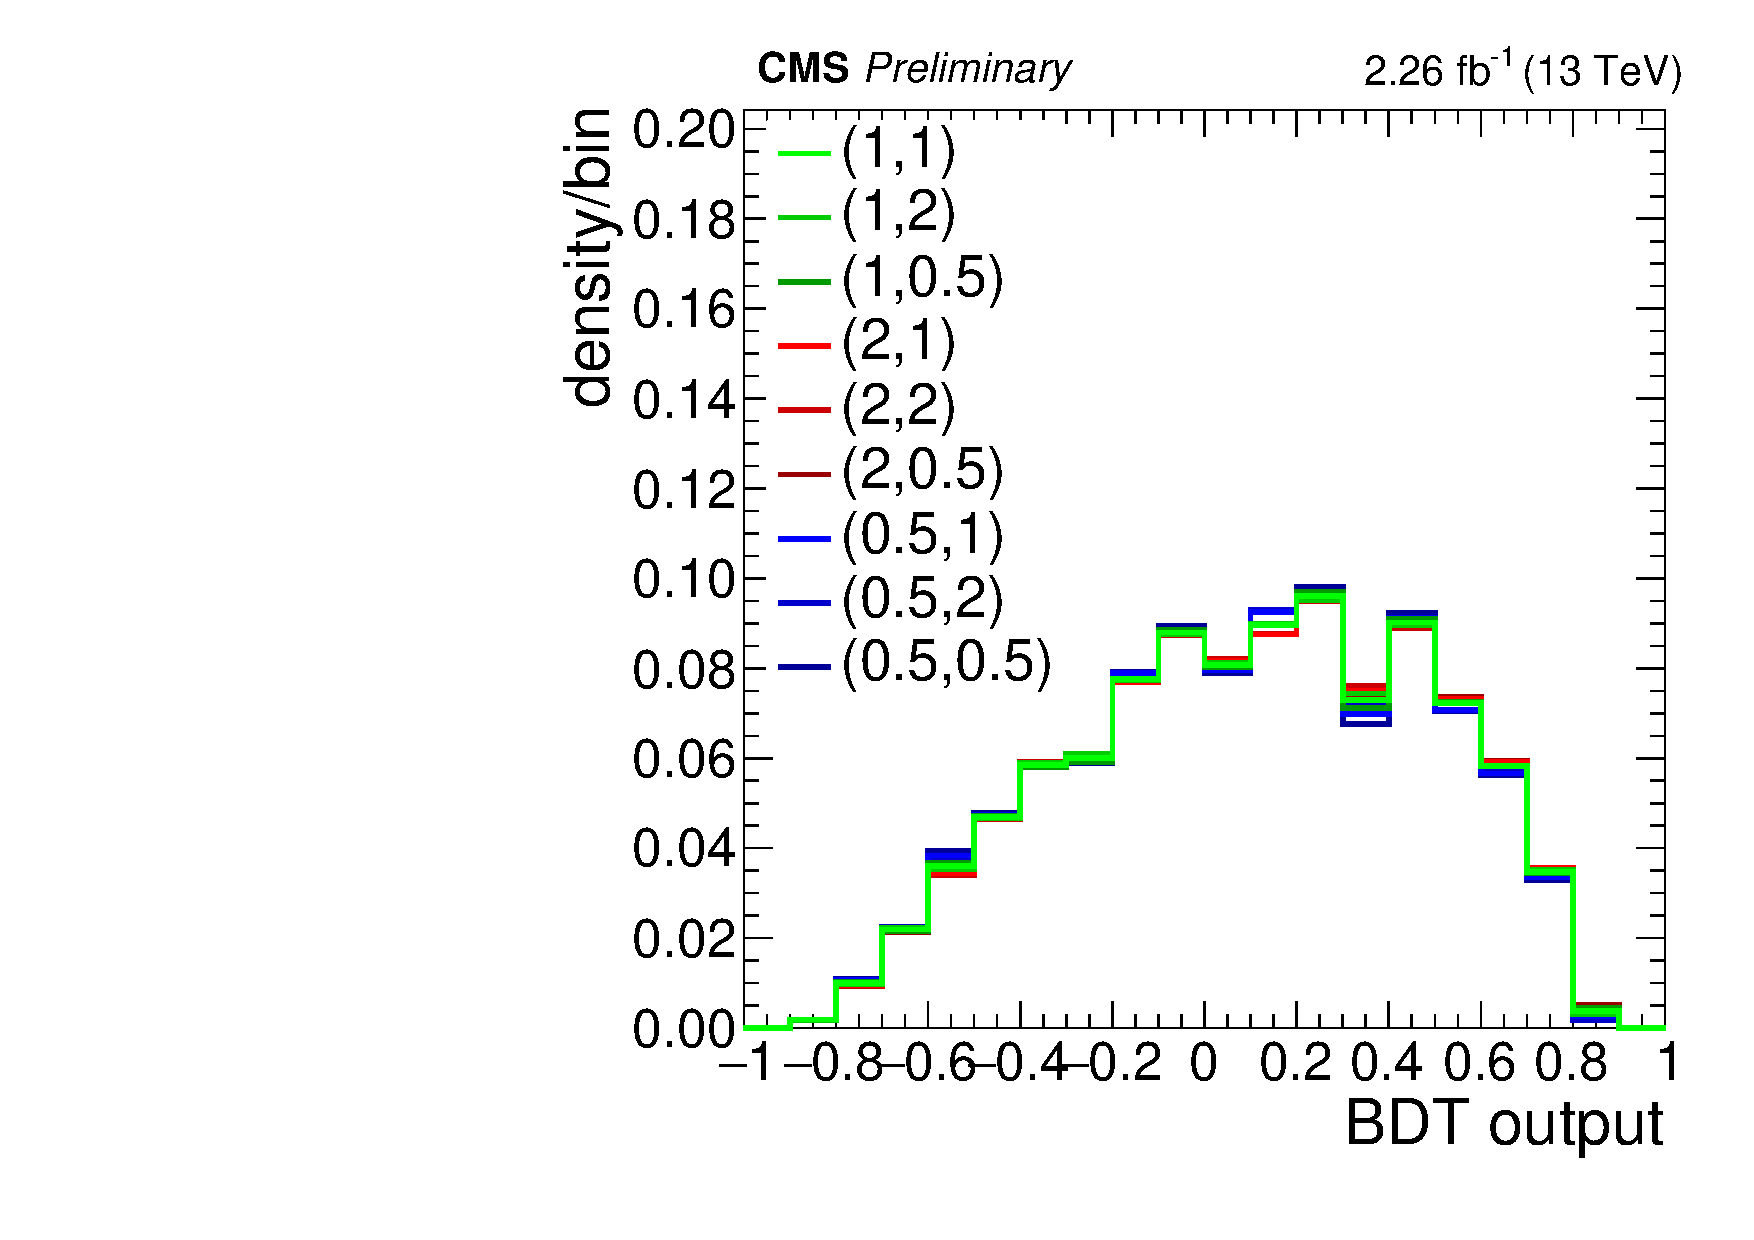
\includegraphics[width=0.35\textwidth]{plots_irreduciblebkg/2lss/muR_muF_ttW/kinMVA_2lss_ttbar}
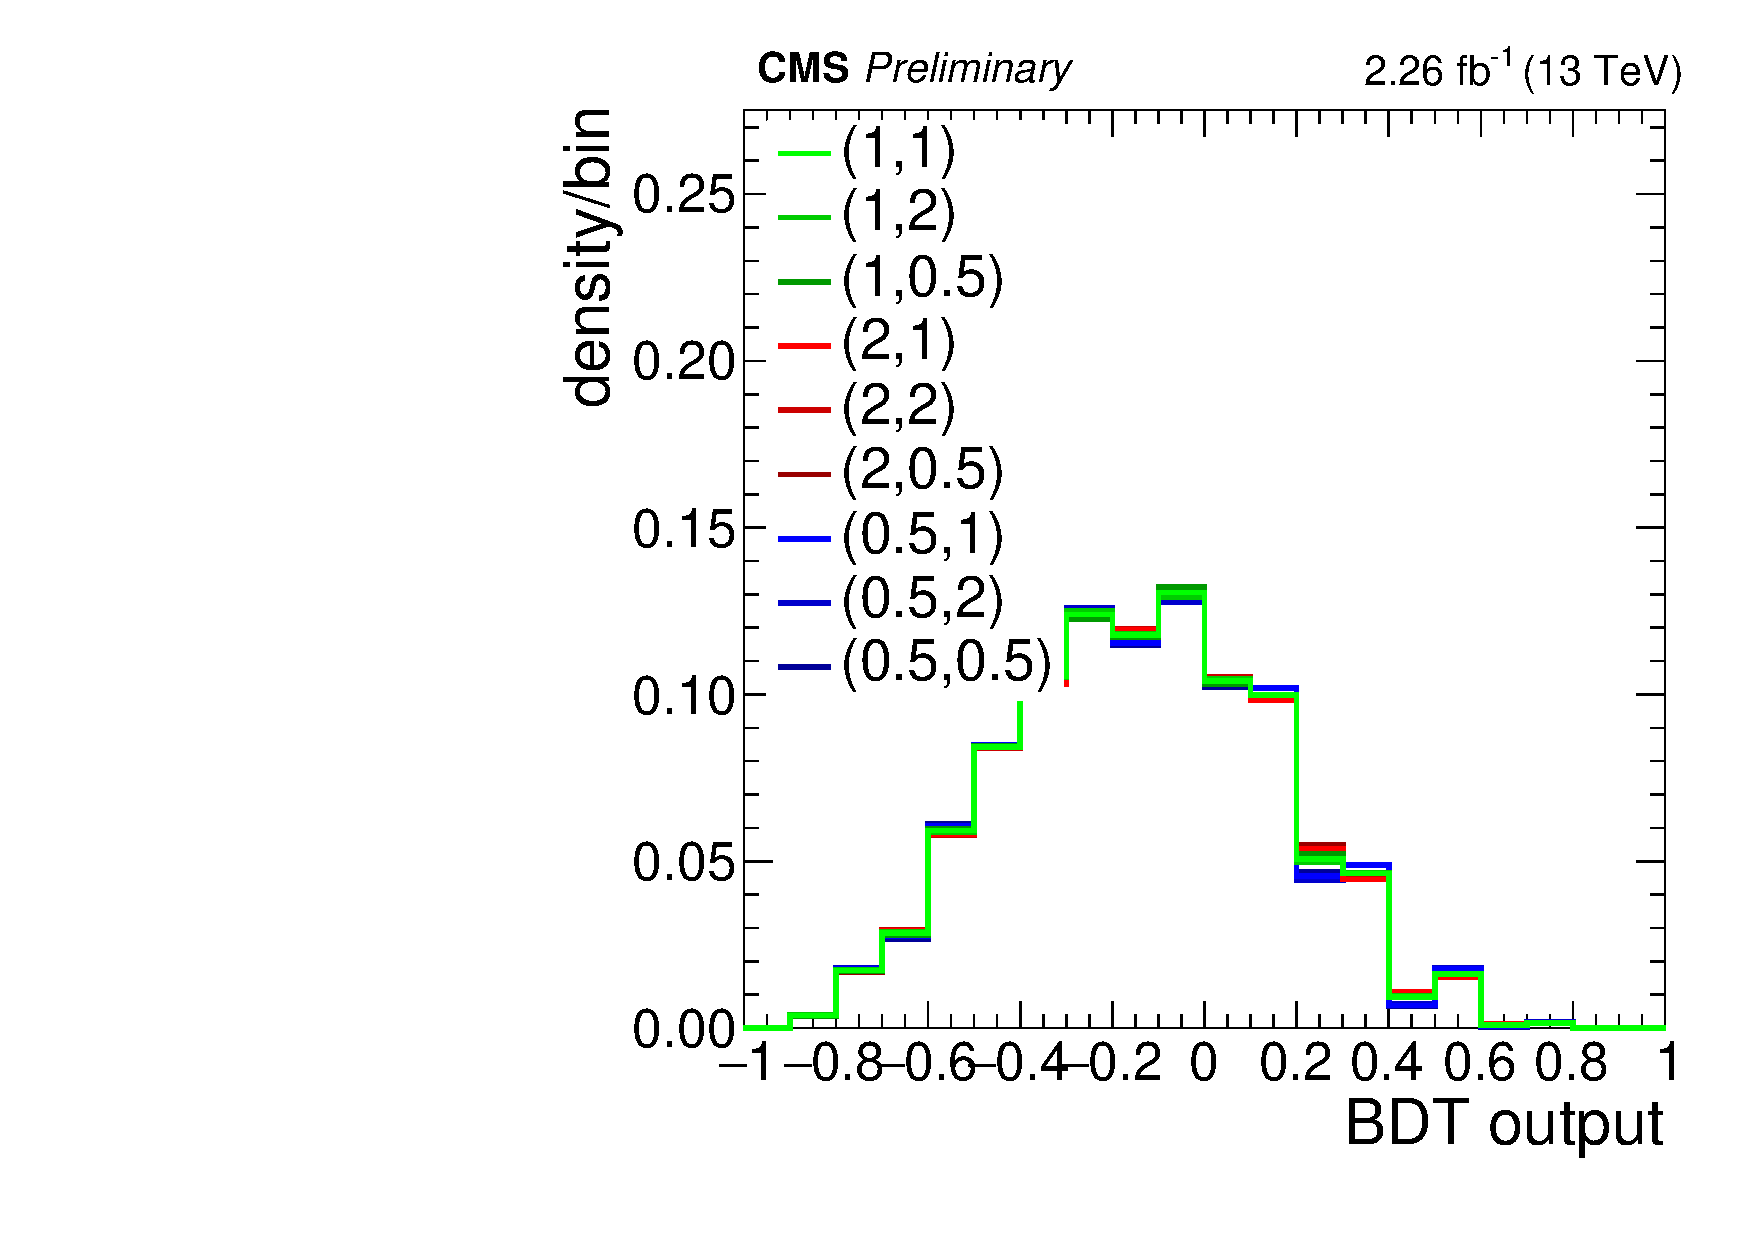
\includegraphics[width=0.35\textwidth]{plots_irreduciblebkg/2lss/muR_muF_ttW/kinMVA_2lss_ttV}
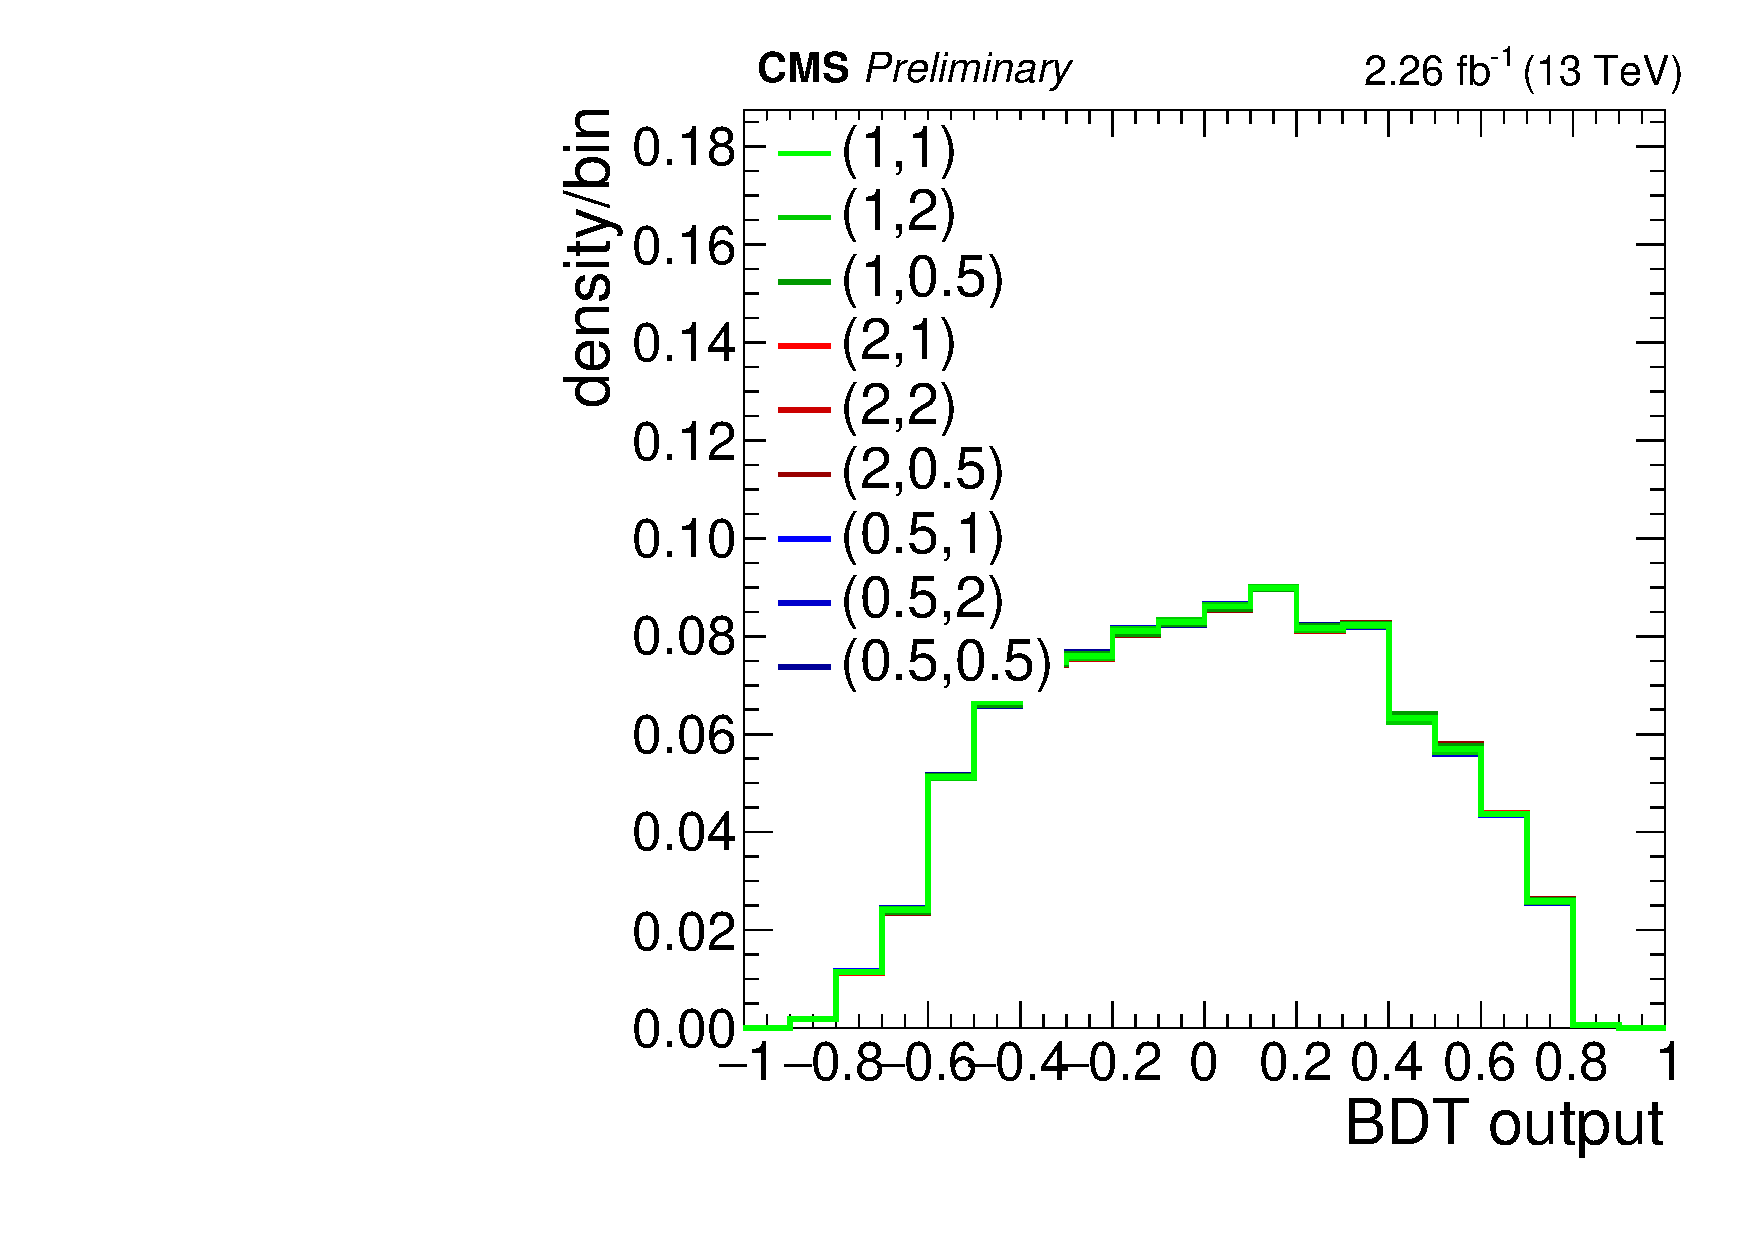
\includegraphics[width=0.35\textwidth]{plots_irreduciblebkg/2lss/muR_muF_ttZ/kinMVA_2lss_ttbar}
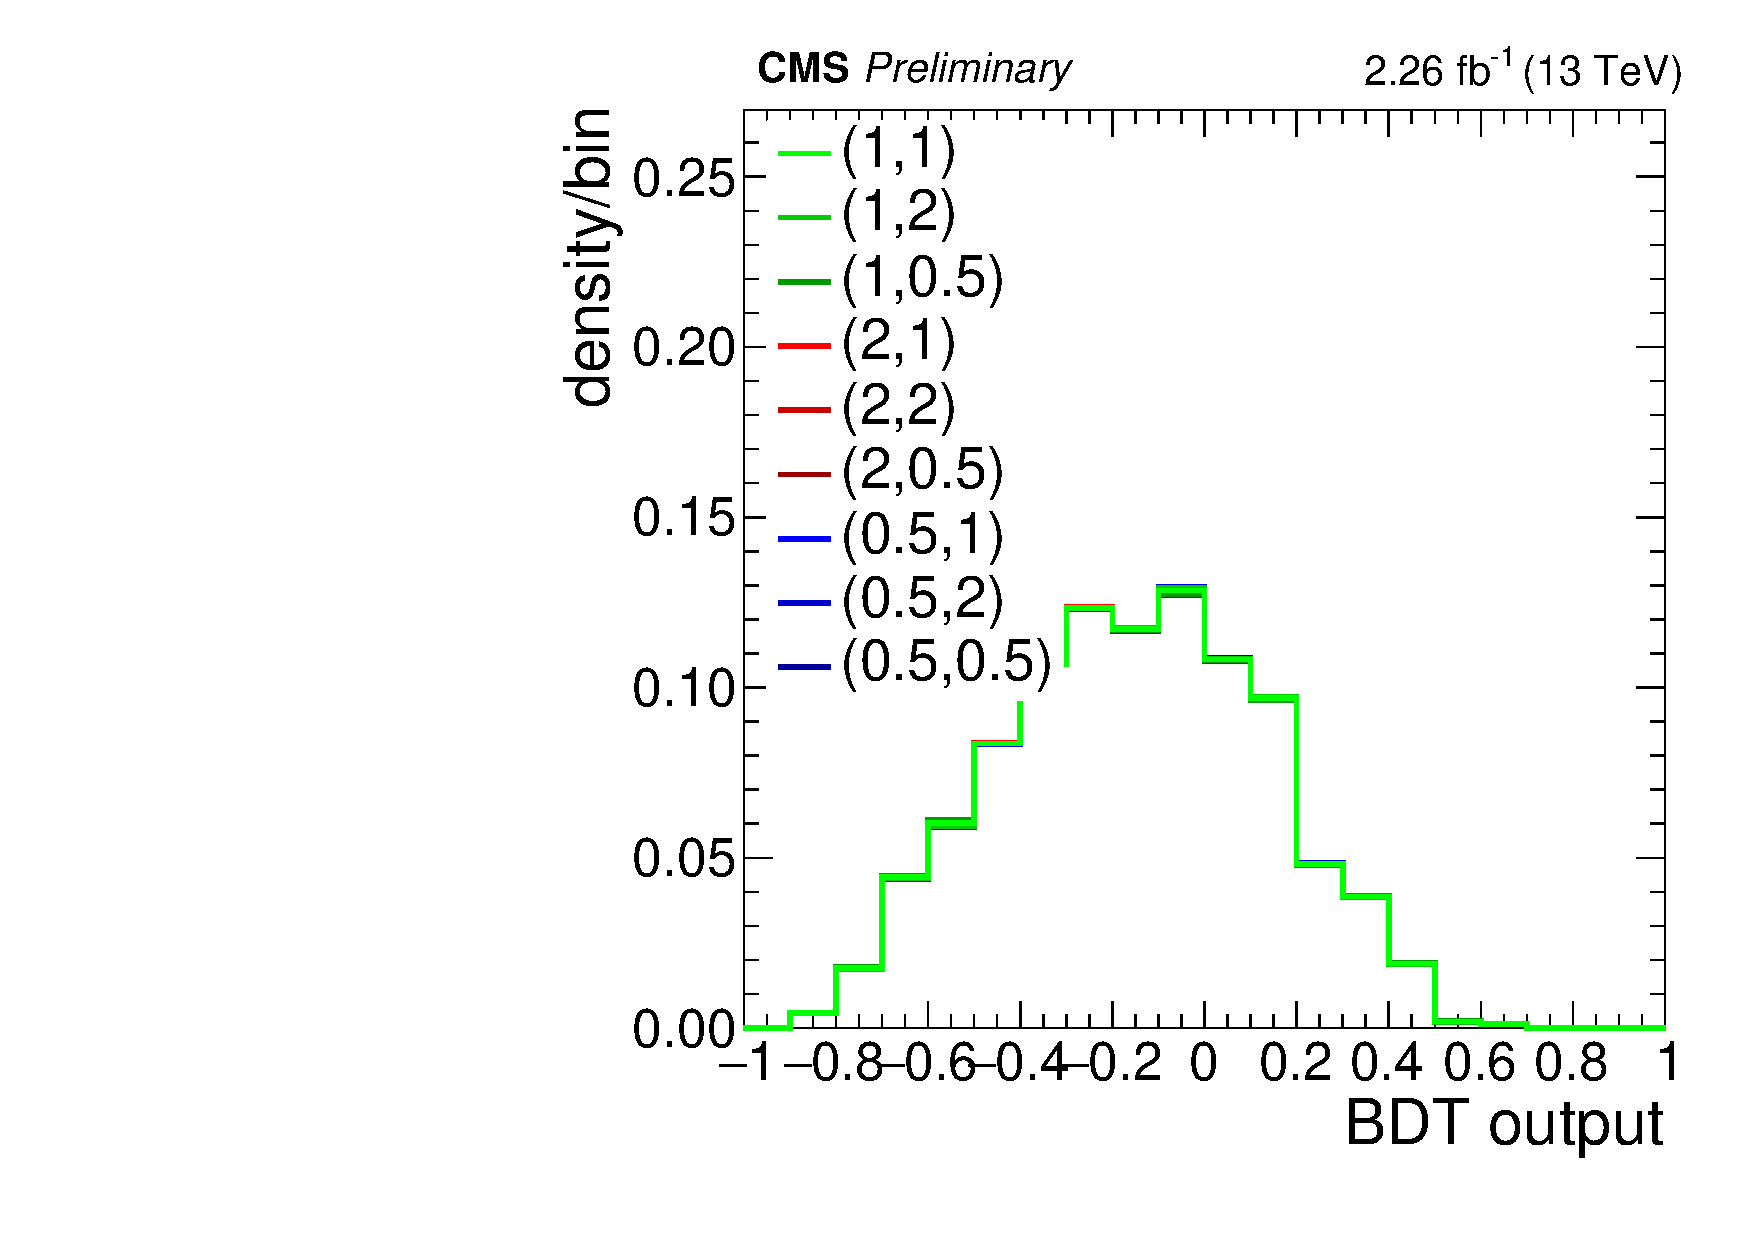
\includegraphics[width=0.35\textwidth]{plots_irreduciblebkg/2lss/muR_muF_ttZ/kinMVA_2lss_ttV}
	\caption{The BDT output distribution of the ttW and ttZ, shown for the training against ttbar 
	(left) and ttV (right) in the two same sign leptons final state, with variations of the
	renormalization and factorization scale included in order to estimate the shape uncertainties.}
	\label{fig:TTVScaleonBDTshape2lss}
\end{figure}

\begin{figure}[htb]
	\centering 
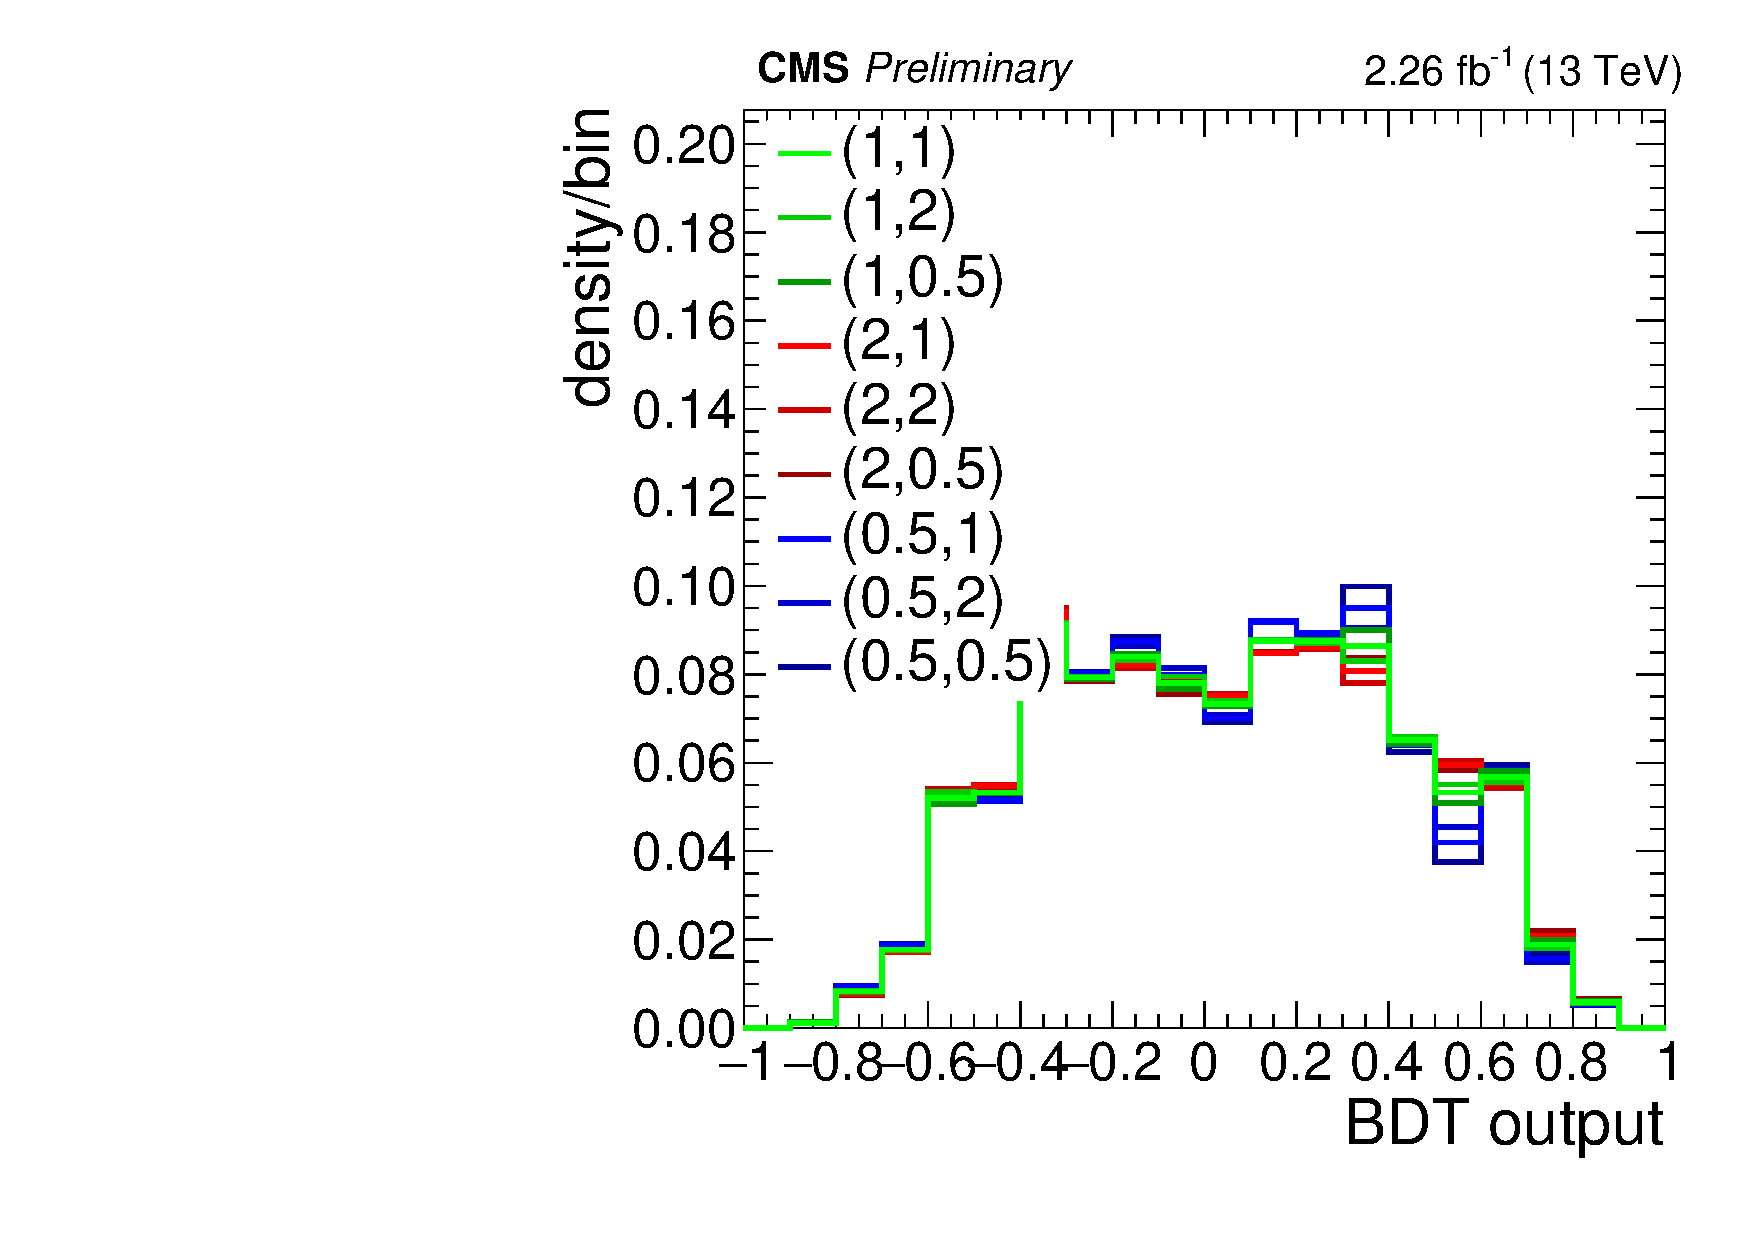
\includegraphics[width=0.35\textwidth]{plots_irreduciblebkg/3l/muR_muF_ttW/kinMVA_3l_ttbar}
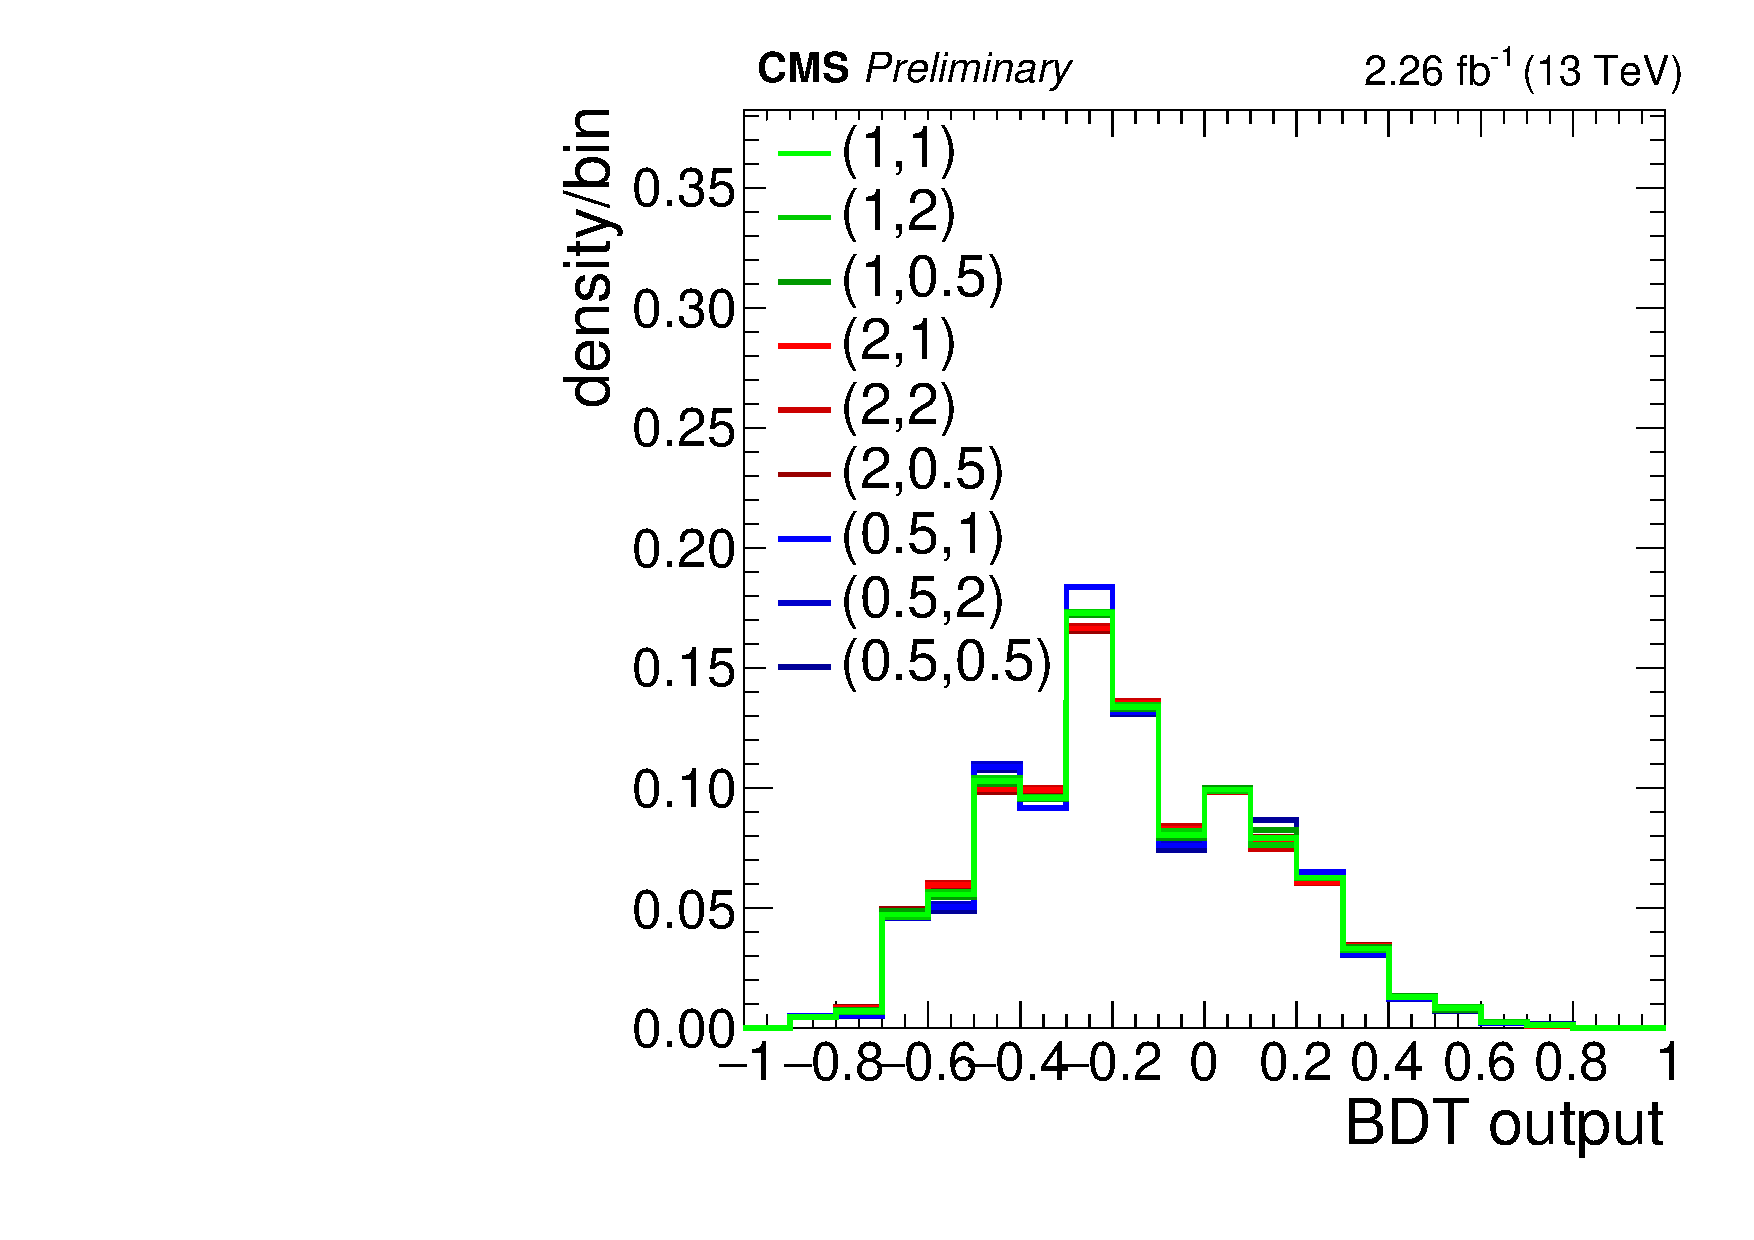
\includegraphics[width=0.35\textwidth]{plots_irreduciblebkg/3l/muR_muF_ttW/kinMVA_3l_ttV}
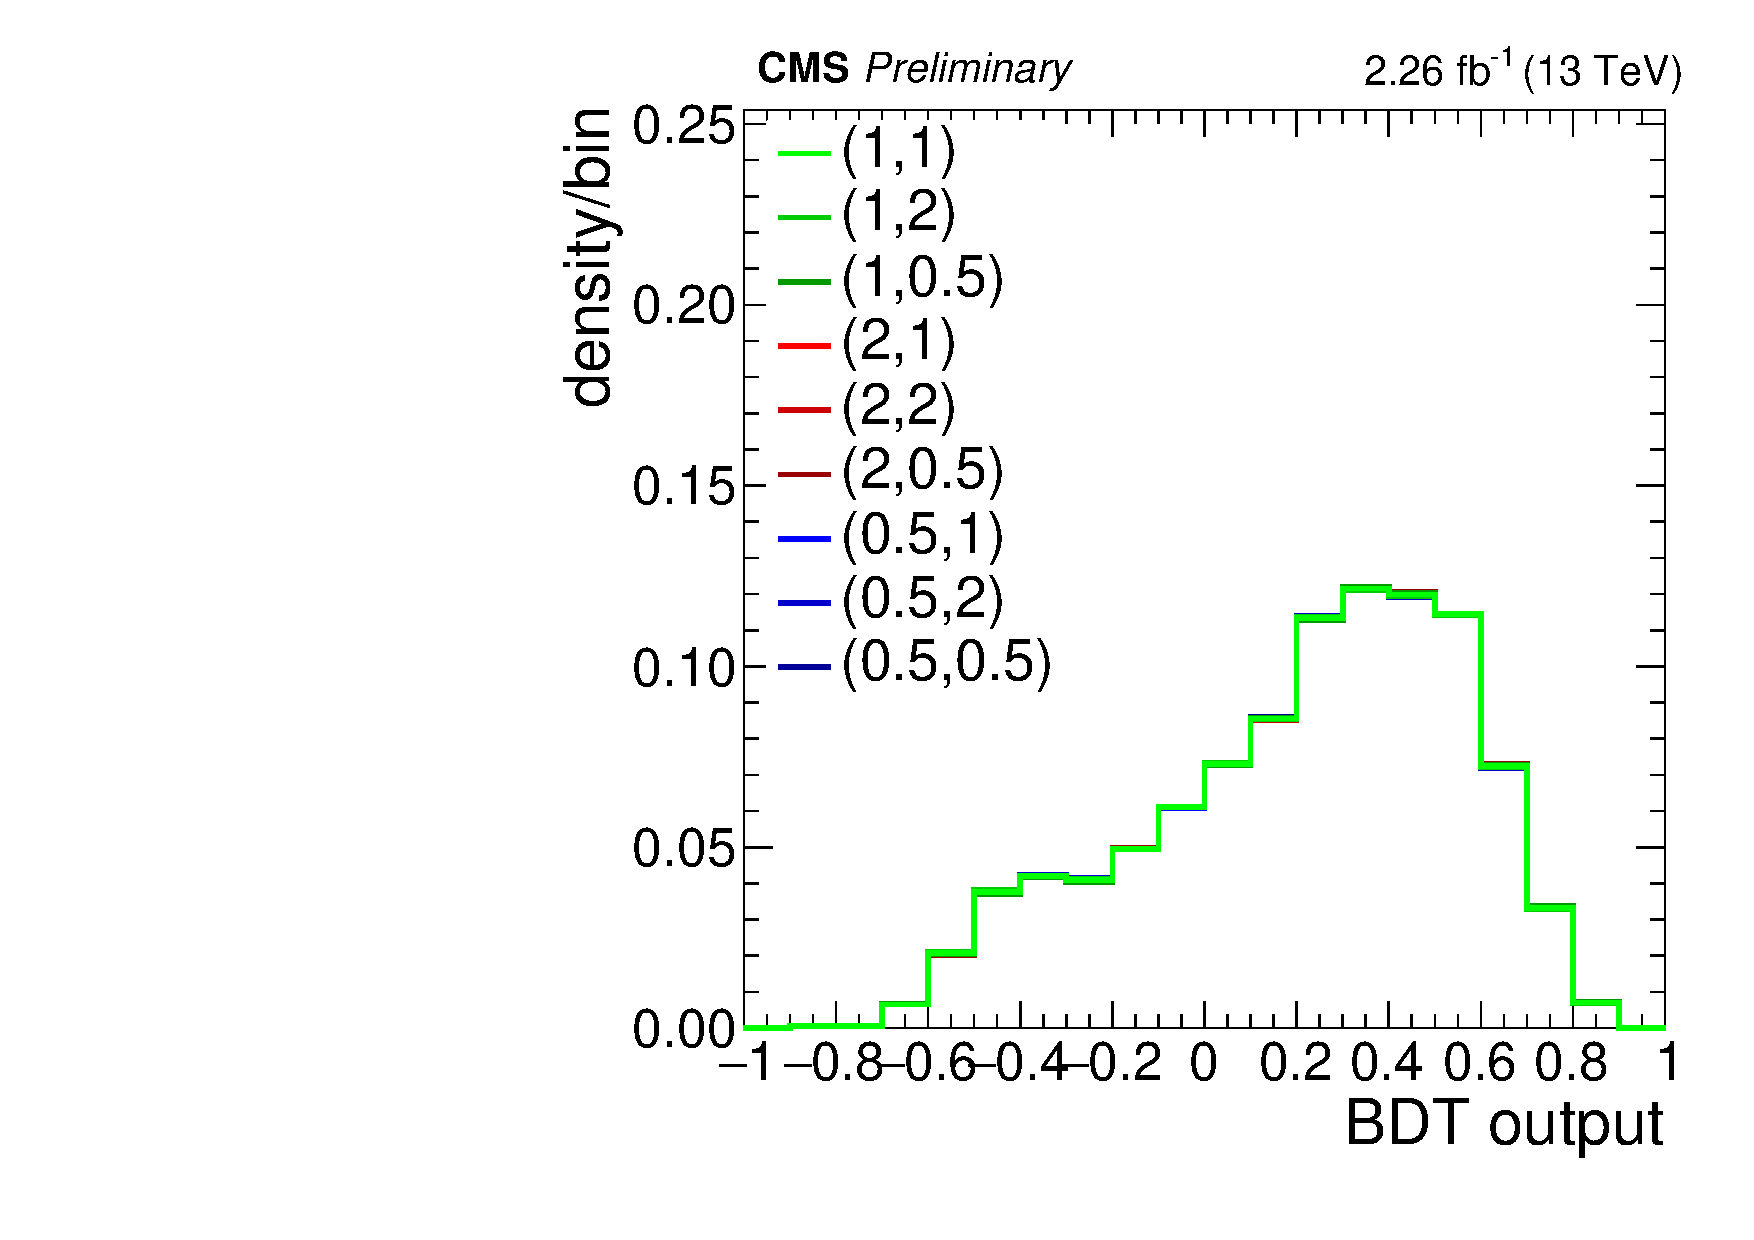
\includegraphics[width=0.35\textwidth]{plots_irreduciblebkg/3l/muR_muF_ttZ/kinMVA_3l_ttbar}
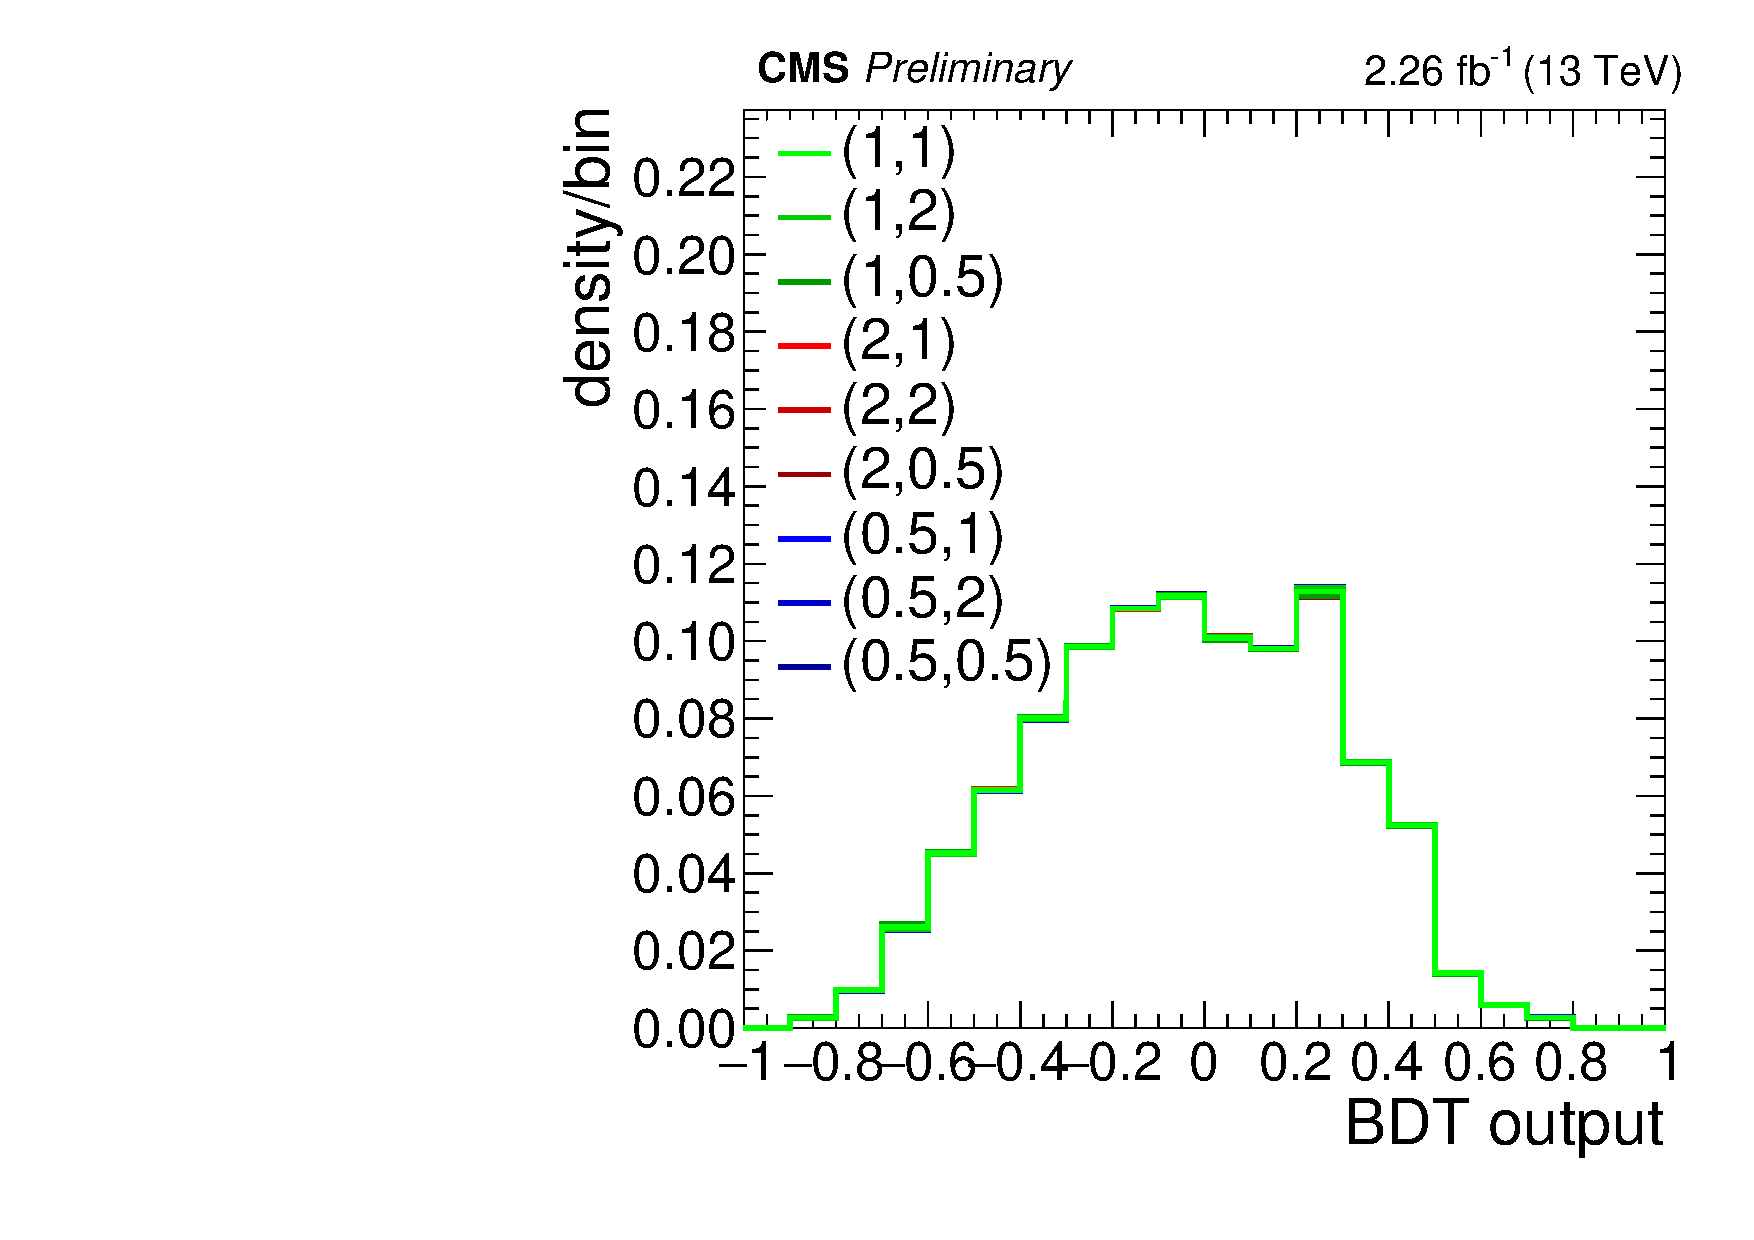
\includegraphics[width=0.35\textwidth]{plots_irreduciblebkg/3l/muR_muF_ttZ/kinMVA_3l_ttV}
	\caption{The BDT output distribution of the ttW and ttZ, shown for the training against ttbar 
	(left) and ttV (right) in the three lepton final state, with the variations of the
	renormalization and factorization scale included in order to estimate the shape uncertainties.}
	\label{fig:TTVScaleonBDTshape3l}
\end{figure}


The cross section for the $\ttbar\gamma^*$ process with $\gamma^*\to\ell^+\ell^-$ process becomes large for decreasing virtuality of the $\gamma^*$, i.e. for small invariant masses of the dilepton pair. While in the analysis we reject events with low mass dileptons, the $\ttbar\gamma^*$ process can still contribute as a background when one of the two leptons is not reconstructed; this in particular can happen in kinematic configurations where the conversion is very asymmetric and one of the two leptons has transverse momentum below the acceptance.\\
Since the nominal $\ttbar\Z$ MC sample is generated with the
requirement $m_{\ell^+\ell^-} > 10\GeV$, to estimate this background
we rely on an additional $\ttbar\gamma^*$ MC sample generated in the
remaining part of the phase space. This additional sample is generated
with LO \textsc{Madgraph}, and the details of the generation and
normalization can be find here~\cite{lowMll}.

In the case of electrons, in addition to the $\ttbar\gamma^*$
background there is a similar topology of events from $\ttbar\gamma$
production where the photon converts early in the detector material,
one conversion electron is not reconstructed and the remaining can
then be misidentified as prompt electron\footnote{If both electrons
  are reconstructed, then the conversion veto applied in the electron
  selection will reject both.}. This background, despite being
reducible, is not covered by the reducible background estimation
obtained extrapolating from leptons failing the MVA requirement,
described later in section \ref{sec:fakerate}, since the electron
arising from the converted photon will be isolated, unlike non-prompt
electrons from hadron decays or misidentified charged hadrons. We
therefore rely on simulations normalized to NLO QCD cross section from Madraph5\_aMC@NLO.\\

In addition to the experimental uncertainties, we assign a systematic uncertainty of $30\%$ to the overall normalization of $\ttbar\,\gamma$ and a systematic uncertainty of $50\%$ on the overall normalization of $\ttbar\gamma^*$.
